%Version 3.1 December 2024
% See section 11 of the User Manual for version history
%
%%%%%%%%%%%%%%%%%%%%%%%%%%%%%%%%%%%%%%%%%%%%%%%%%%%%%%%%%%%%%%%%%%%%%%
%%                                                                 %%
%% Please do not use \input{...} to include other tex files.       %%
%% Submit your LaTeX manuscript as one .tex document.              %%
%%                                                                 %%
%% All additional figures and files should be attached             %%
%% separately and not embedded in the \TeX\ document itself.       %%
%%                                                                 %%
%%%%%%%%%%%%%%%%%%%%%%%%%%%%%%%%%%%%%%%%%%%%%%%%%%%%%%%%%%%%%%%%%%%%%

%%\documentclass[referee,sn-basic]{sn-jnl}% referee option is meant for double line spacing

%%=======================================================%%
%% to print line numbers in the margin use lineno option %%
%%=======================================================%%

%%\documentclass[lineno,pdflatex,sn-basic]{sn-jnl}% Basic Springer Nature Reference Style/Chemistry Reference Style

%%=========================================================================================%%
%% the documentclass is set to pdflatex as default. You can delete it if not appropriate.  %%
%%=========================================================================================%%

%%\documentclass[sn-basic]{sn-jnl}% Basic Springer Nature Reference Style/Chemistry Reference Style

%%Note: the following reference styles support Namedate and Numbered referencing. By default the style follows the most common style. To switch between the options you can add or remove “Numbered” in the optional parenthesis. 
%%The option is available for: sn-basic.bst, sn-chicago.bst%  
 
%%\documentclass[pdflatex,sn-nature]{sn-jnl}% Style for submissions to Nature Portfolio journals
%%\documentclass[pdflatex,sn-basic]{sn-jnl}% Basic Springer Nature Reference Style/Chemistry Reference Style
% sn-jnl loads hyperref; float must precede it for algorithm/caption links.
\RequirePackage{float}
\documentclass[pdflatex,sn-mathphys-num]{sn-jnl}% Math and Physical Sciences Numbered Reference Style
% The approved vector figures include PDF 1.7 resources.
\ifdefined\pdfminorversion\pdfminorversion=7\fi
%%\documentclass[pdflatex,sn-mathphys-ay]{sn-jnl}% Math and Physical Sciences Author Year Reference Style
%%\documentclass[pdflatex,sn-aps]{sn-jnl}% American Physical Society (APS) Reference Style
%%\documentclass[pdflatex,sn-vancouver-num]{sn-jnl}% Vancouver Numbered Reference Style
%%\documentclass[pdflatex,sn-vancouver-ay]{sn-jnl}% Vancouver Author Year Reference Style
%%\documentclass[pdflatex,sn-apa]{sn-jnl}% APA Reference Style
%%\documentclass[pdflatex,sn-chicago]{sn-jnl}% Chicago-based Humanities Reference Style

%%%% Standard Packages
%%<additional latex packages if required can be included here>

\usepackage{graphicx}%
\usepackage{multirow}%
\usepackage{amsmath,amssymb,amsfonts}%
\usepackage{amsthm}%
\usepackage[title]{appendix}%
\usepackage{xcolor}%
\usepackage{textcomp}%
\usepackage{manyfoot}%
\usepackage{booktabs}%
\usepackage{array}
\usepackage{makecell}
\usepackage{colortbl}
\usepackage{makecell}
\usepackage{algorithm}%
\usepackage{algorithmicx}%
\usepackage{algpseudocode}%
\usepackage{listings}%
\usepackage[normalem]{ulem}
\usepackage{siunitx}
\usepackage{tabularx}
\usepackage{url}
\newcommand{\mname}{SpectraFlow}
\usepackage{hyperref}
% Keep the PDF outline at section/subsection level; paragraph labels are prose.
\hypersetup{bookmarksdepth=2}
%% Float placement tuning: keep large figures near their references
%% (prevents big full-width figures from piling up at the end of the document)
\renewcommand{\topfraction}{0.9}
\renewcommand{\bottomfraction}{0.9}
\renewcommand{\textfraction}{0.07}
\renewcommand{\floatpagefraction}{0.7}
\setcounter{topnumber}{3}
\setcounter{bottomnumber}{3}
\setcounter{totalnumber}{6}
\makeatletter
\setlength{\@fptop}{0pt}% align full-page (float-page) figures to the top
\makeatother

%%%%

%%%%%=============================================================================%%%%
%%%%  Remarks: This template is provided to aid authors with the preparation
%%%%  of original research articles intended for submission to journals published 
%%%%  by Springer Nature. The guidance has been prepared in partnership with 
%%%%  production teams to conform to Springer Nature technical requirements. 
%%%%  Editorial and presentation requirements differ among journal portfolios and 
%%%%  research disciplines. You may find sections in this template are irrelevant 
%%%%  to your work and are empowered to omit any such section if allowed by the 
%%%%  journal you intend to submit to. The submission guidelines and policies 
%%%%  of the journal take precedence. A detailed User Manual is available in the 
%%%%  template package for technical guidance.
%%%%%=============================================================================%%%%

%% as per the requirement new theorem styles can be included as shown below
\theoremstyle{thmstyleone}%
\newtheorem{theorem}{Theorem}%  meant for continuous numbers
%%\newtheorem{theorem}{Theorem}[section]% meant for sectionwise numbers
%% optional argument [theorem] produces theorem numbering sequence instead of independent numbers for Proposition
\newtheorem{proposition}[theorem]{Proposition}% 
%%\newtheorem{proposition}{Proposition}% to get separate numbers for theorem and proposition etc.

\theoremstyle{thmstyletwo}%
\newtheorem{example}{Example}%
\newtheorem{remark}{Remark}%

\theoremstyle{thmstylethree}%
\newtheorem{definition}{Definition}%

\raggedbottom
%%\unnumbered% uncomment this for unnumbered level heads

\begin{document}

\title[SpectraFlow]{SpectraFlow: bidirectional infrared--Raman translation and molecular representation learning}
%%=============================================================%%
%% GivenName	-> \fnm{Joergen W.}
%% Particle	-> \spfx{van der} -> surname prefix
%% FamilyName	-> \sur{Ploeg}
%% Suffix	-> \sfx{IV}
%% \author*[1,2]{\fnm{Joergen W.} \spfx{van der} \sur{Ploeg} 
%%  \sfx{IV}}\email{iauthor@gmail.com}
%%=============================================================%%

\author[1,2]{\fnm{Jiaqing} \sur{Xie}}\email{xiejiaqing@pjlab.org.cn}


\author[3]{\fnm{Zhuo} \sur{Yang}}\email{yzachary1551@gmail.com}


\author[1,4]{\fnm{Ben} \sur{Gao}}\email{gaoben@pjlab.org.cn}

\author[6]{\fnm{Shuaike} \sur{Shen}}

 

\author[1,5]{\fnm{Tianfan} \sur{Fu}}\email{futianfan@nju.edu.cn}

\author[1]{\fnm{Yuqiang} \sur{Li}}\email{liyuqiang@pjlab.org.cn}
% \author[1,2]{\fnm{Third} \sur{Author}}\email{iiiauthor@gmail.com}


\affil[1]{\orgname{Shanghai Artificial Intelligence Laboratory}, \orgaddress{\city{Shanghai}, \country{China}}}

\affil[2]{\orgname{Fudan University}, \orgaddress{\city{Shanghai}, \country{China}}}


\affil[3]{\orgname{Southeast University}, \orgaddress{\city{Nanjing}, \state{Jiangsu}, \country{China}}}

\affil[4]{\orgdiv{The Institute for Advanced Studies}, \orgname{Wuhan University}, \orgaddress{\city{Wuhan}, \state{Hubei}, \country{China}}}

\affil[5]{\orgdiv{State Key Laboratory for Novel Software Technology at Nanjing University, School of Computer Science}, \orgname{Nanjing University}, \orgaddress{\city{Nanjing}, \state{Jiangsu}, \country{China}}}

\affil[6]{\orgname{Carnegie Mellon University}, \orgaddress{\city{Pittsburgh}, \state{Pennsylvania}, \country{USA}}}

\abstract{Infrared and Raman spectra encode complementary molecular vibrations, but paired measurements are scarce and distinct selection rules complicate cross-modal prediction. Here we introduce SpectraFlow, a conditional flow-matching model for bidirectional spectral translation. A one-dimensional Transformer learns a source-conditioned velocity field with peak-weighted and shape-sensitive objectives and eight-step deterministic integration. Across three computed-spectrum benchmarks, SpectraFlow reduces infrared-to-Raman root-mean-square error by approximately 20--29\% relative to the strongest evaluated baseline. Training on a single source domain also lowers mean absolute error across seven held-out chemical domains. Experimental-input and cross-library tests retain partial spectral correspondence but reveal substantial domain shifts. Frozen embeddings improve molecular-descriptor prediction over raw spectra and provide task-dependent gains when combined with molecular fingerprints. These results support cross-modal spectral learning for normalized spectral completion and reusable molecular representations, while identifying experimental calibration and peak fidelity as remaining challenges.}

%%\pacs[JEL Classification]{D8, H51}

%%\pacs[MSC Classification]{35A01, 65L10, 65L12, 65L20, 65L70}

\enlargethispage{2\baselineskip}
\maketitle

\noindent
Vibrational spectroscopy links molecular structure to experimentally observable signals. Infrared (IR) absorption and Raman scattering probe the same molecular normal modes through different responses: changes in dipole moment and polarizability, respectively~\cite{Hashimoto_2019,Chang_2022,Meng_2025}. Their selection rules make the two modalities complementary. A vibration that is weak or inactive in one spectrum may be prominent in the other; in centrosymmetric molecules, IR and Raman activity are mutually exclusive. Access to both modalities can therefore aid band assignment and the characterization of molecular bonding and symmetry~\cite{yuan2025qme14s,wang2025diffspectra,wang2025molspectra}.

Paired measurements are nevertheless difficult to obtain at scale. Public IR and Raman libraries have developed largely independently, and Raman acquisition can be limited by weak scattering, fluorescence and sample damage~\cite{Chan_2005,Sasmaz_2015,Wei_2015,Shipp_2017}. Quantum-chemical calculations provide paired spectra, but their cost and sensitivity to computational approximations, molecular conformation and environment limit direct correspondence with measurements~\cite{zou2023deep,liang2025dataset,Laury_2012,Barone_2014,Bloino_2015}. Predicting one modality from the other could help complete spectral records when paired data are unavailable. Such predictions must be interpreted as learned estimates: selection rules can hide information in the source, so the target spectrum is not generally determined by a simple rescaling of source intensities.

Cross-modal learning must resolve narrow peaks while using relationships across the wavenumber axis. Existing work has explored learned IR--Raman correspondence~\cite{yang2024cross}, alongside broader approaches to learning from molecular spectra~\cite{lu2025vib2mol,cai2025deep,kanakala2024spectra,alberts2025setting,su2025language}. Two questions remain central to this task: how well a learned mapping transfers across chemical and measurement domains, and whether translation produces representations useful beyond spectral reconstruction. The shared molecular origin of the two modalities motivates testing cross-modal prediction as an objective for molecular representation learning~\cite{zhu2026spectrogen}.

Here we introduce \mname, a conditional flow-matching framework for bidirectional IR--Raman translation (Fig.~\ref{fig:pipeline}). A one-dimensional Transformer learns a source-conditioned velocity field over ordered wavenumber sequences. Peak weighting, derivative matching and local optimal transport emphasize spectral morphology, while deterministic integration produces a target prediction and intermediate model states. We evaluate translation on three computed-spectrum benchmarks, transfer from the ViBench-QM9 source domain to seven held-out domains, and performance under experimental-input and cross-library shifts. We also test whether frozen translation-trained features support molecular-descriptor prediction. These evaluations distinguish reconstruction accuracy, domain transfer and representation utility, while treating the learned trajectory as a computational path rather than physical molecular dynamics.

\begin{figure}[htbp]
    \centering
    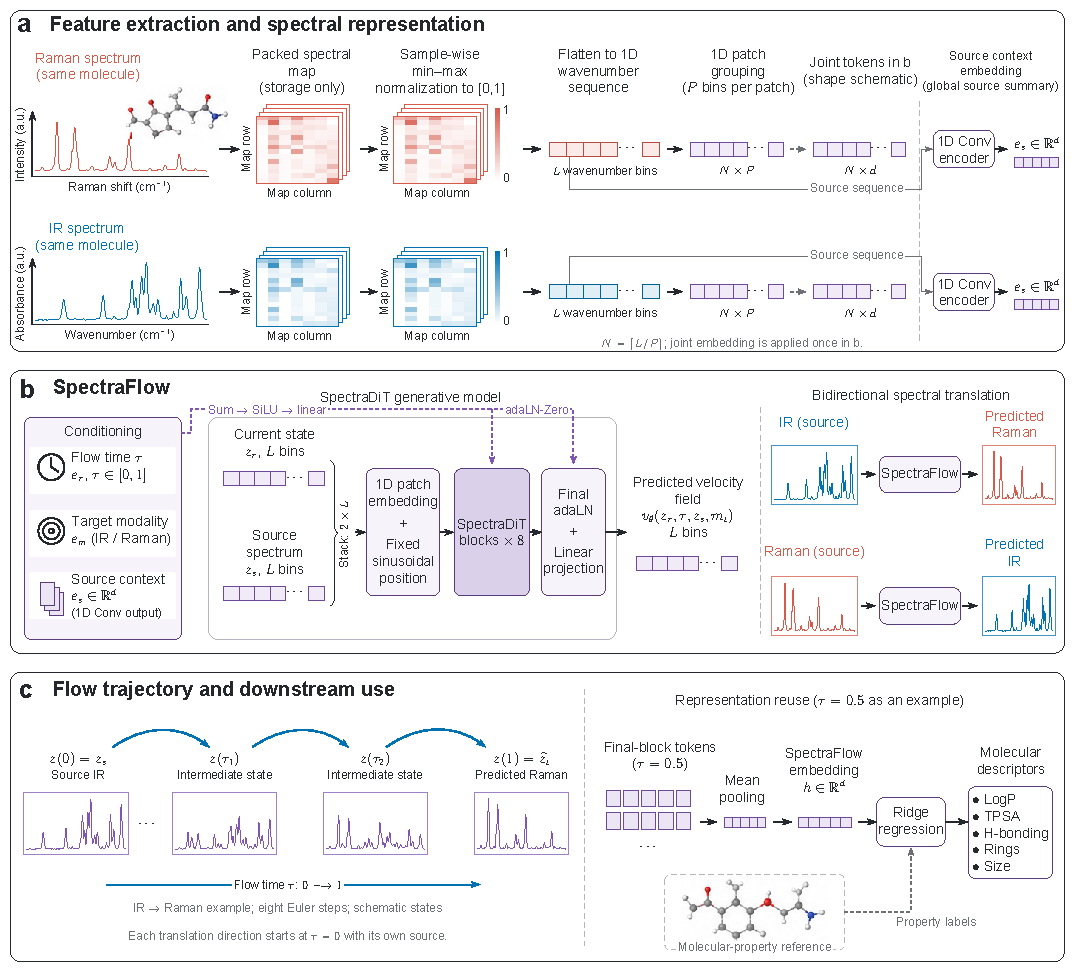
\includegraphics[width=\linewidth]{figs/Figure_1_reference_tikz.pdf}
    \caption{\textbf{Overview of \mname\ for bidirectional IR--Raman translation.}
    \textbf{a,} Paired spectra are normalized sample-wise and flattened into ordered wavenumber sequences; heatmaps depict per-spectrum storage grids. Patch grouping and token dimensions are schematic. The learned joint embedding is applied once to the stacked channels in b. A separate one-dimensional convolutional encoder summarizes the source sequence.
    \textbf{b,} The current state and source spectrum, $[z_\tau,z_s]$, pass through a joint one-dimensional patch embedding, fixed sinusoidal positions, eight SpectraDiT blocks and an output head. Summed time, modality and source-context embeddings undergo SiLU activation and an affine projection before conditioning adaptive layer normalization. Separate checkpoints implement the two translation directions.
    \textbf{c,} Four schematic states illustrate IR$\rightarrow$Raman translation with eight Euler steps. Integration starts from the source at $\tau=0$ and ends at the predicted target at $\tau=1$. Final-block tokens at the source-generated midpoint $\tau=0.5$ are mean-pooled for ridge-regression probes. Molecular structures supply property labels, not translator inputs. Spectra, heatmaps and intermediate states are schematic.}
    \label{fig:pipeline}
\end{figure}
\label{sec1}


\section*{Results}

\subsection*{Conditional transport between vibrational modalities}

\mname\ learns a velocity field conditioned on the source spectrum, current spectral state, flow time and target modality (Fig.~\ref{fig:pipeline}). Spectra are normalized sample-wise and represented as ordered one-dimensional sequences. A patch embedding groups neighbouring wavenumber bins, fixed sinusoidal positions encode their order, and eight SpectraDiT blocks exchange information across the sequence. Time, modality and global source features condition the blocks through adaptive layer normalization. Separate checkpoints implement IR$\rightarrow$Raman and Raman$\rightarrow$IR translation.

Training matches the velocity along an interpolation between paired source and target spectra. Peak-weighted reconstruction, derivative matching and local optimal transport provide additional endpoint supervision. At inference, eight Euler steps evolve the source into a normalized target prediction. Output projection enforces the interval $[0,1]$. Intermediate states expose the numerical transformation without implying a physical trajectory.

\subsection*{Translation accuracy and transfer across chemical domains}

\begin{figure}[htbp]
    \centering
    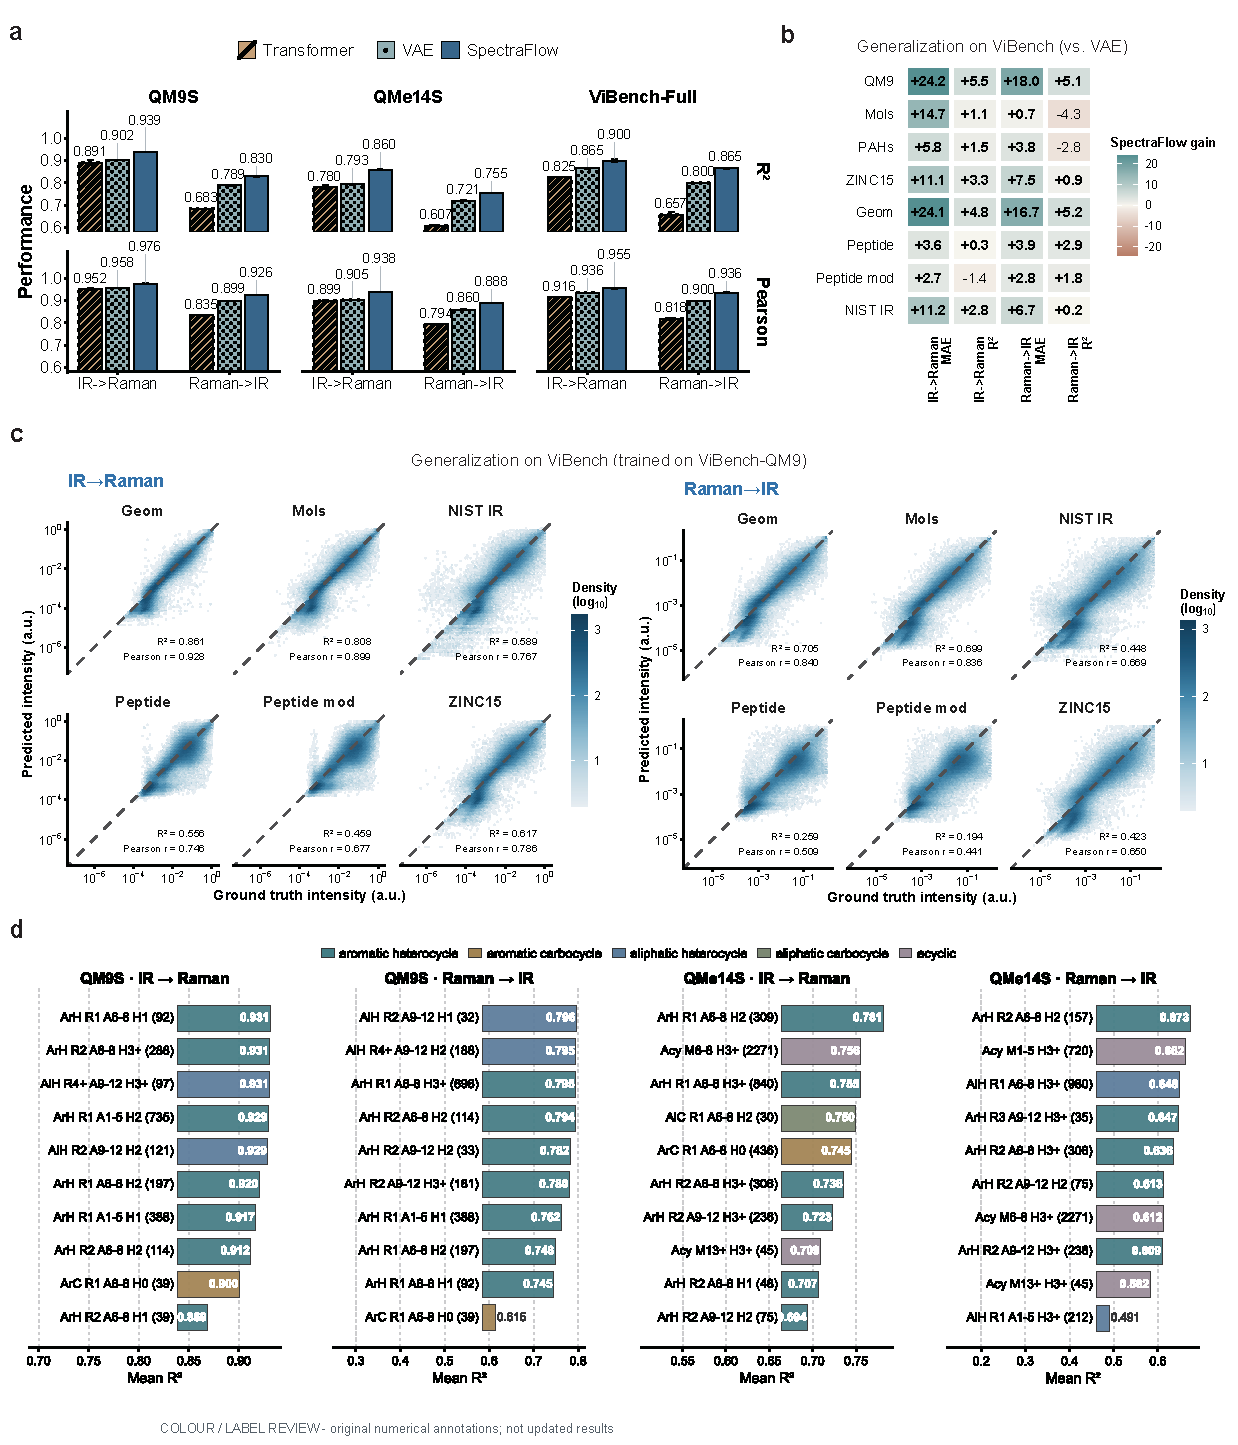
\includegraphics[width=\linewidth]{figs/results/result_1_draw_arial.pdf}
    \caption{\textbf{In-distribution performance and cross-dataset generalization of \mname.}
\textbf{a,} Translation performance of the Transformer, VAE, and \mname\ on QM9S, QMe14S, and ViBench-Full in both directions.
\textbf{b,} Cross-dataset gains of \mname\ over VAE across eight ViBench domains after training on ViBench-QM9, reported as MAE reduction and $R^2$ improvement.
\textbf{c,} Predicted versus ground-truth intensity distributions on six held-out ViBench domains without per-dataset tuning.
\textbf{d,} In-distribution $R^2$ stratified by Murcko scaffold class for QM9S and QMe14S; classes contain at least 30 test molecules.}
    \label{fig:quantitative_result}
\end{figure}

\begin{table}[!htb]
\centering
\caption{\textbf{Bidirectional translation on QM9S, QMe14S and ViBench-Full.}
Values are mean $\pm$ s.d. over four model-initialization seeds on fixed test partitions. VAE and Transformer denote the reconstruction baselines specified in Methods; \mname\ uses conditional flow matching with a one-dimensional SpectraDiT backbone. Bold denotes the best mean. Asterisks denote adjusted $p<0.05$ in two-sided paired Wilcoxon tests against the strongest baseline, with Holm--Bonferroni correction as described in Methods.
Predictions are rescaled using the paired target's minimum and maximum for evaluation on the dataset's native intensity scale. RMSE magnitudes are therefore not comparable across datasets; the large QMe14S Raman values reflect its intensity scale. This reporting convention requires target statistics and does not demonstrate prediction of unknown absolute intensities. Per-spectrum $R^2$ and Pearson $r$ are invariant to the shared affine rescaling.
}
\label{tab:reconstruction}
\scriptsize
\setlength{\tabcolsep}{3.6pt}
\renewcommand{\arraystretch}{1.15}
\begin{tabular}{llcccc}
\toprule
Task & Model & R$^2 \uparrow$ & Pearson $\uparrow$ & RMSE $\downarrow$ & SSIM $\uparrow$ \\
\midrule
\multicolumn{6}{l}{\bfseries\itshape  QM9S\ (\# test: 19,474)} \\
\midrule
\multirow{3}{*}{IR $\rightarrow$ Raman}
& VAE       & $0.902_{\pm 0.001}$ & $0.958_{\pm 0.000}$ & $6.664_{\pm 0.037}$ & $0.940_{\pm 0.002}$ \\
& Transformer & $0.891_{\pm 0.012}$ & $0.952_{\pm 0.006}$ & $6.921_{\pm 0.355}$ & $0.933_{\pm 0.007}$ \\
& \mname\ & $\mathbf{0.939_{\pm 0.001}}$* & $\mathbf{0.976_{\pm 0.001}}$* & $\mathbf{5.129_{\pm 0.036}}$* & $\mathbf{0.963_{\pm 0.001}}$* \\
\cmidrule(lr){1-6}
\multirow{3}{*}{Raman $\rightarrow$ IR}
& VAE & $0.789_{\pm 0.002}$ & $0.899_{\pm 0.001}$ & $8.222_{\pm 0.036}$ & $0.873_{\pm 0.002}$ \\
& Transformer & $0.683_{\pm 0.002}$ & $0.835_{\pm 0.002}$ & $10.178_{\pm 0.050}$ & $0.783_{\pm 0.002}$ \\
&\mname & $\mathbf{0.830_{\pm 0.003}}$* & $\mathbf{0.926_{\pm 0.001}}$* & $\mathbf{7.007_{\pm 0.044}}$* & $\mathbf{0.908_{\pm 0.001}}$* \\
\midrule
\multicolumn{6}{l}{\bfseries\itshape QMe14S\ (\# test: 27,916)} \\
\midrule
\multirow{3}{*}{IR $\rightarrow$ Raman}
& VAE       & $0.793_{\pm 0.004}$ & $0.905_{\pm 0.000}$ & $8727_{\pm 168.4}$  &$0.879_{\pm 0.002}$  \\
& Transformer & $0.780_{\pm 0.009}$  & $0.899_{\pm 0.005}$  & $8972_{\pm 15.39}$  & $0.868_{\pm 0.005}$  \\
& \mname\ & $\mathbf{0.860_{\pm 0.001}}$*  & $\mathbf{0.938_{\pm 0.000}}$*  & $\mathbf{6949_{\pm 129.6}}$*  & $\mathbf{0.921_{\pm 0.000}}$* \\
\cmidrule(lr){1-6}
\multirow{3}{*}{Raman $\rightarrow$ IR}
& VAE       & $0.721_{\pm 0.002}$ & $0.860_{\pm 0.001}$ & $4.084_{\pm 0.024}$ & $0.823_{\pm 0.001}$ \\
& Transformer & $0.607_{\pm 0.002}$ & $0.794_{\pm 0.002}$ & $4.877_{\pm 0.011}$ & $0.729_{\pm 0.004}$ \\
& \mname & $\mathbf{0.755_{\pm 0.001}}$* & $\mathbf{0.888_{\pm 0.000}}$* & $\mathbf{3.630_{\pm 0.043}}$* & $\mathbf{0.863_{\pm 0.001}}$* \\
\midrule
\multicolumn{6}{l}{\bfseries\itshape ViBench-Full\ (\# test: 13,793)} \\
\midrule
\multirow{3}{*}{IR $\rightarrow$ Raman}
& VAE       & $0.865_{\pm 0.001}$  & $0.936_{\pm 0.000}$  & $0.031_{\pm 0.000}$  & $0.926_{\pm 0.001}$ \\
& Transformer &  $0.825_{\pm 0.000}$  & $0.916_{\pm 0.001}$  & $0.035_{\pm 0.000}$  & $0.902_{\pm 0.001}$ \\
&\mname\  &  $\mathbf{0.900_{\pm 0.006}}$* & $\mathbf{0.955_{\pm 0.003}}$* & $\mathbf{0.022_{\pm 0.001}}$* & $\mathbf{0.948_{\pm 0.003}}$* \\
\cmidrule(lr){1-6}
\multirow{3}{*}{Raman $\rightarrow$ IR}
& VAE       &   $0.800_{\pm 0.000}$  & $0.900_{\pm 0.000}$  & $0.033_{\pm 0.000}$  & $0.887_{\pm 0.002}$\\
& Transformer &  $0.657_{\pm 0.011}$  & $0.818_{\pm 0.005}$  & $0.046_{\pm 0.000}$  & $0.789_{\pm 0.003}$ \\
& \mname\  &  $\mathbf{0.865_{\pm 0.002}}$* & $\mathbf{0.936_{\pm 0.001}}$* & $\mathbf{0.022_{\pm 0.001}}$* & $\mathbf{0.928_{\pm 0.002}}$* \\

\bottomrule
\end{tabular}
\renewcommand{\arraystretch}{1.0}
\end{table}

\mname\ has the highest mean $R^2$, Pearson correlation and SSIM, and the lowest RMSE, among the three models in all six dataset--direction comparisons (Table~\ref{tab:reconstruction}). For IR$\rightarrow$Raman, $R^2$ reaches $0.939$, $0.860$ and $0.900$ on QM9S, QMe14S and ViBench-Full, respectively. Relative to VAE, the strongest baseline by RMSE in each case, these results correspond to approximately $23\%$, $20\%$ and $29\%$ lower RMSE. Raman$\rightarrow$IR follows the same ranking on these benchmarks: $R^2$ increases from $0.789$ to $0.830$ on QM9S, from $0.721$ to $0.755$ on QMe14S, and from $0.800$ to $0.865$ on ViBench-Full.

A one-pass SpectraDiT-Direct comparison provides context for the role of the backbone (Supplementary Table~\ref{tab:direct-ablation}). Direct retains the velocity-network architecture but predicts a residual with one network evaluation. It reaches $R^2=0.910$ for IR$\rightarrow$Raman and $0.806$ for Raman$\rightarrow$IR on QM9S, compared with $0.939$ and $0.830$ for eight-step Flow. Direct therefore retains much of the endpoint accuracy. Its shorter optimization budget and lower endpoint-loss coefficient, however, mean that this comparison does not isolate the effect of integration.

For transfer evaluation, models are trained on the ViBench-QM9 source domain and evaluated on its supplied QM9 test set and seven held-out domains: Mols, PAHs, ZINC15, GEOM, Peptide, Peptide-mod and NIST-IR~\citep{lu2025vib2mol}. No domain-specific fine-tuning or additional split is applied. \mname\ lowers MAE relative to VAE on all eight evaluation sets in both directions (Fig.~\ref{fig:quantitative_result}b; Supplementary Table~\ref{tab:vae-vibraflow-main}). The mean relative reductions across the eight sets are approximately $12.2\%$ for IR$\rightarrow$Raman and $7.5\%$ for Raman$\rightarrow$IR. IR$\rightarrow$Raman reductions approach $24\%$ on QM9 and GEOM.

The transfer advantage depends on the metric. $R^2$ improves on seven of eight sets for IR$\rightarrow$Raman and six of eight for Raman$\rightarrow$IR. It decreases for IR$\rightarrow$Raman on Peptide-mod and for Raman$\rightarrow$IR on Mols and PAHs despite lower MAE. On PAHs, IR$\rightarrow$Raman $R^2$ remains negative for both models. Intensity-density plots illustrate the variation across domains, and scaffold-stratified results show variation within QM9S and QMe14S (Fig.~\ref{fig:quantitative_result}c,d). Scaffold classes describe subgroups of random test partitions; they do not constitute scaffold-disjoint evaluation.

The endpoint-supervision comparison increases the probability of computing the endpoint loss from $0.1$ to $0.5$. In the reported sixteen comparisons, MAE decreases and $R^2$ and Pearson correlation increase, with a median relative MAE reduction of approximately $8.1\%$. Because the loss is reweighted by the inverse sampling probability, its expected coefficient remains fixed. This comparison therefore changes the frequency and stochasticity of endpoint supervision, rather than simply increasing its expected weight.

\subsection*{Experimental inputs and cross-library evaluation}

Two evaluations examine measurement-domain shifts (Fig.~\ref{fig:experimental_validation}). The first applies a QM9S-trained IR$\rightarrow$Raman model directly to experimental NIST IR spectra and compares predictions with computed QM9S Raman targets. Molecular matching yields 84 overlaps: 76 stereochemistry-aware exact matches and eight connectivity-only matches. Median Pearson correlations are $0.42$ and $0.40$, respectively. Selected exact-match examples reach $r=0.673$, $0.671$ and $0.644$, but the full distribution shows substantially lower correspondence than the controlled computed-spectrum benchmarks. This tests a change in the source measurement domain, rather than establishing generalization to previously unseen molecular identities.

The second evaluation trains a separate model on cross-library OpenSpecy/RRUFF pairs and tests it on 147 pairs from held-out RRUFF identifiers. The development pool contains 590 identifiers and the external test contains 147 identifiers spanning 135 mineral names. The median test correlation is $0.31$ for raw spectra and $0.34$ after baseline correction of predictions and references. Selected records labelled rutile, cassiterite and staurolite reach correlations of $0.953$, $0.942$ and $0.852$. These selected cases show what is attainable for some records; they do not represent average test performance. Identifier matching also does not ensure common specimens or acquisition conditions, and 72 test mineral names occur in the development pool under different identifiers.

The NIST error profile localizes the largest mean normalized discrepancies to approximately $2800$--$3200\,\mathrm{cm}^{-1}$ (Fig.~\ref{fig:experimental_validation}e). The shaded $2200$--$2450\,\mathrm{cm}^{-1}$ interval is a reference region; the error profile alone does not establish the cause of any discrepancy. These evaluations quantify incomplete correspondence under measurement shifts and motivate calibration with paired experimental spectra.

\begin{figure}[htbp]
    \centering
    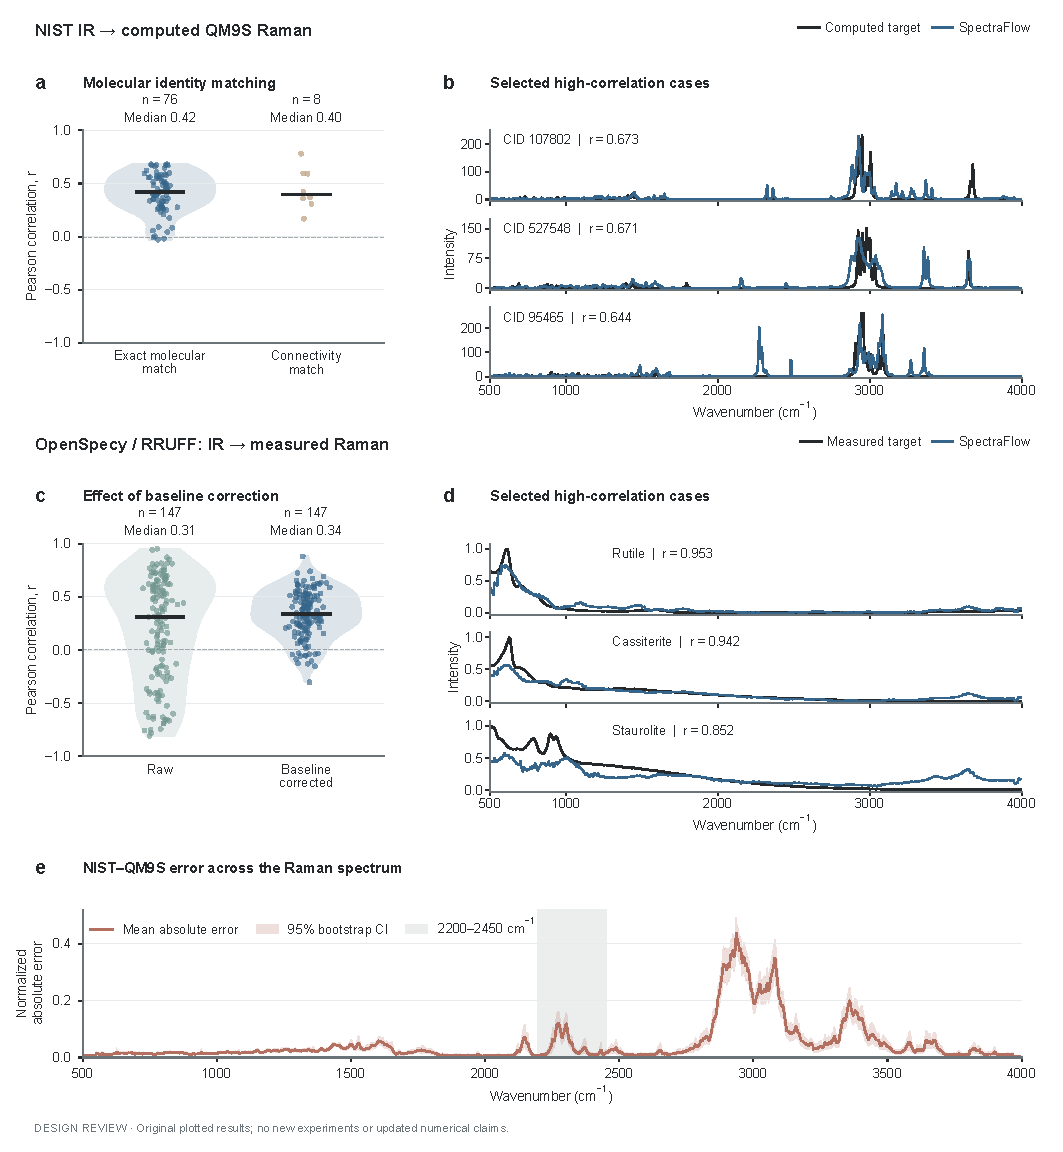
\includegraphics[width=0.98\linewidth]{figs/results/result_4_draw_arial.pdf}
    \caption{\textbf{Experimental-input and cross-library IR$\rightarrow$Raman transfer of \mname.}
\textbf{a,} Pearson correlations for experimental NIST IR inputs against identity-matched computed QM9S Raman targets.
\textbf{b,} Three selected high-correlation NIST--QM9S predictions; targets are computed Raman spectra.
\textbf{c,} Pearson distributions for 147 held-out OpenSpecy/RRUFF pairs before and after baseline correction.
\textbf{d,} Selected high-correlation cross-library predictions against measured Raman targets. The selected cases in b and d do not summarize population-average accuracy.
\textbf{e,} Wavenumber-resolved normalized absolute error across the NIST--QM9S matches; shading denotes the 95\% bootstrap confidence interval. The grey interval marks $2200$--$2450\,\mathrm{cm}^{-1}$ for reference.}
    \label{fig:experimental_validation}
\end{figure}

\subsection*{Peak-resolved errors and intermediate spectral states}

\begin{figure}[htbp]
    \centering
    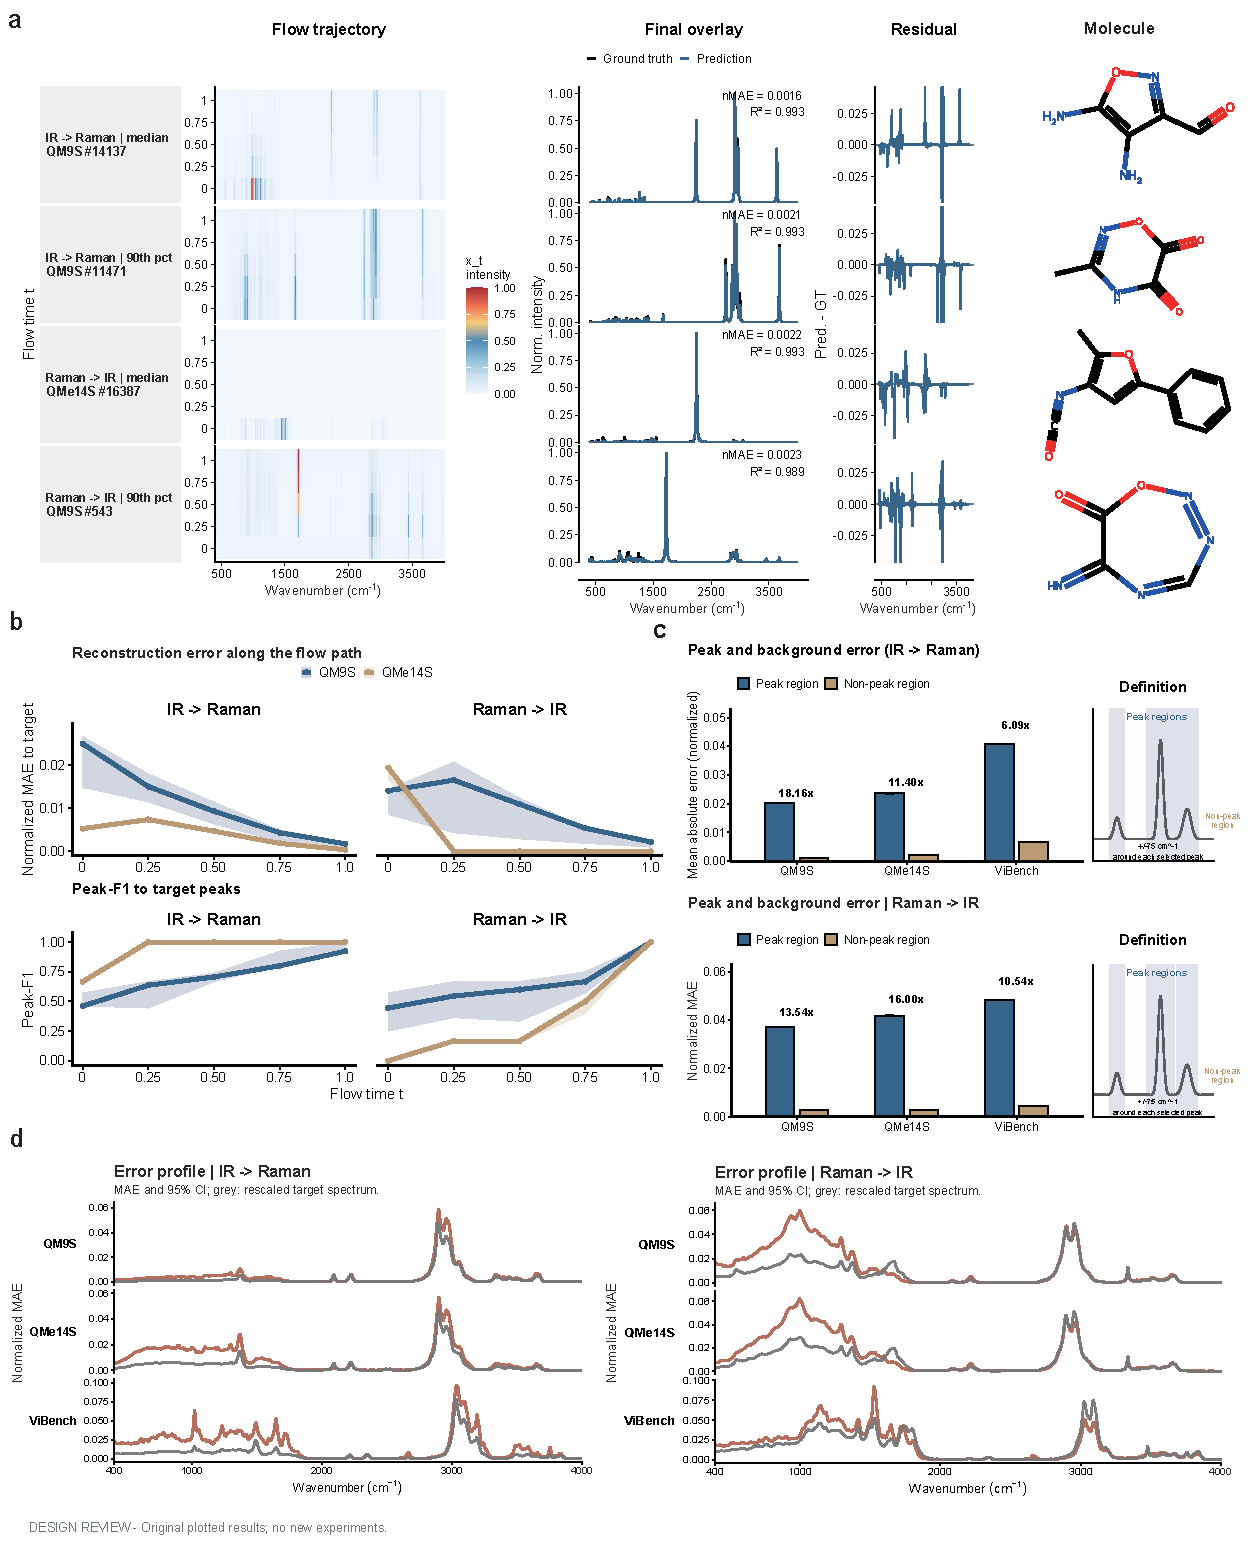
\includegraphics[width=0.97\linewidth]{figs/results/result_2_draw_polished.pdf}
    \caption{\textbf{Learned conversion trajectories and peak-localized prediction error.}
\textbf{a,} Four selected cases: IR$\rightarrow$Raman, QM9S \#14137 and \#11471; Raman$\rightarrow$IR, QMe14S \#16387 and QM9S \#543. Columns show intermediate spectral states, endpoint overlays, residuals and molecular structures. Black curves denote targets and blue curves predictions.
\textbf{b,} Normalized MAE and peak-F1 along the learned flow path. Colour denotes dataset. Flow time describes the model trajectory, not physical molecular dynamics.
\textbf{c,} Peak-region and background errors for both translation directions. Peak regions span $\pm75\,\mathrm{cm}^{-1}$ around selected target peaks; labels give peak/background error ratios.
\textbf{d,} Wavenumber-resolved normalized MAE and 95\% confidence intervals. Grey curves show mean target spectra rescaled for visual comparison.}
    \label{fig:case_study}
\end{figure}

Residual errors are concentrated near spectral peaks (Fig.~\ref{fig:case_study}c,d). Defining peak regions as the union of $\pm75\,\mathrm{cm}^{-1}$ windows around detected target peaks, the peak-to-background normalized error ratios are $18.2$, $11.4$ and $6.1$ for IR$\rightarrow$Raman on QM9S, QMe14S and ViBench, respectively. The corresponding Raman$\rightarrow$IR ratios are $13.5$, $16.0$ and $10.5$. These ratios describe where errors occur; they do not establish their cause.

A separate peak-matching analysis covers all $19{,}474$ QM9S test spectra. At a $20\,\mathrm{cm}^{-1}$ tolerance, IR$\rightarrow$Raman recovers $80.9\%$ of reference peaks, compared with $68.7\%$ for Raman$\rightarrow$IR (Supplementary Fig.~\ref{fig:qm9s_peak_resolved}). High correlations between matched peak intensities coexist with missed peaks, illustrating why aggregate spectral similarity does not fully describe local fidelity.

Selected trajectories show how predictions develop during integration (Fig.~\ref{fig:case_study}a,b). The illustrated endpoints reach approximately $R^2=0.99$ and normalized MAE of $0.0016$--$0.0023$. Along the plotted paths, target MAE generally decreases and peak-F1 increases, although some intermediate steps temporarily increase error. The states are numerical model outputs and need not correspond to realizable molecular spectra. They complement endpoint metrics by exposing where intensity is redistributed during prediction.

\subsection*{Frozen embeddings support molecular-descriptor prediction}

We next test the representations learned during spectral translation (Fig.~\ref{fig:quantitative_result_3}). A model trained on ViBench-QM9 is frozen, and source-generated final-block features at flow time $\tau=0.5$ are mean-pooled. Dataset-specific ridge probes predict ten RDKit descriptors using five shared random train--test splits. The eight evaluation sets include the QM9 source-domain test set and seven held-out domains. Feature comparisons use raw IR, raw Raman, Flow embeddings, Morgan fingerprints and concatenated Flow--fingerprint features. Molecular structures provide descriptor labels and fingerprints; they are not inputs to the spectral translator.

Flow embeddings make the descriptors more accessible to linear prediction than raw spectra in the reported comparisons (Fig.~\ref{fig:quantitative_result_3}b,c). On GEOM, for example, LogP $R^2$ increases from approximately $0.11$ with raw Raman features to approximately $0.70$ with Flow embeddings. UMAP projections illustrate property-associated organization but are not used as evidence of predictive accuracy (Fig.~\ref{fig:quantitative_result_3}a). Because the downstream probes are fitted within each dataset, the evaluation tests transfer of the frozen encoder rather than zero-shot transfer of a property predictor.

Morgan fingerprints remain a strong reference for descriptors calculated from molecular structure. Adding Flow features yields task-dependent changes, including absolute $R^2$ gains approaching $0.15$ and decreases on other property--dataset pairs (Fig.~\ref{fig:quantitative_result_3}d). Changes are expressed as absolute differences in $R^2$. The mixed gains support complementarity for some linear probes, rather than a uniform advantage from concatenation.

\begin{figure}[htbp]
    \centering
    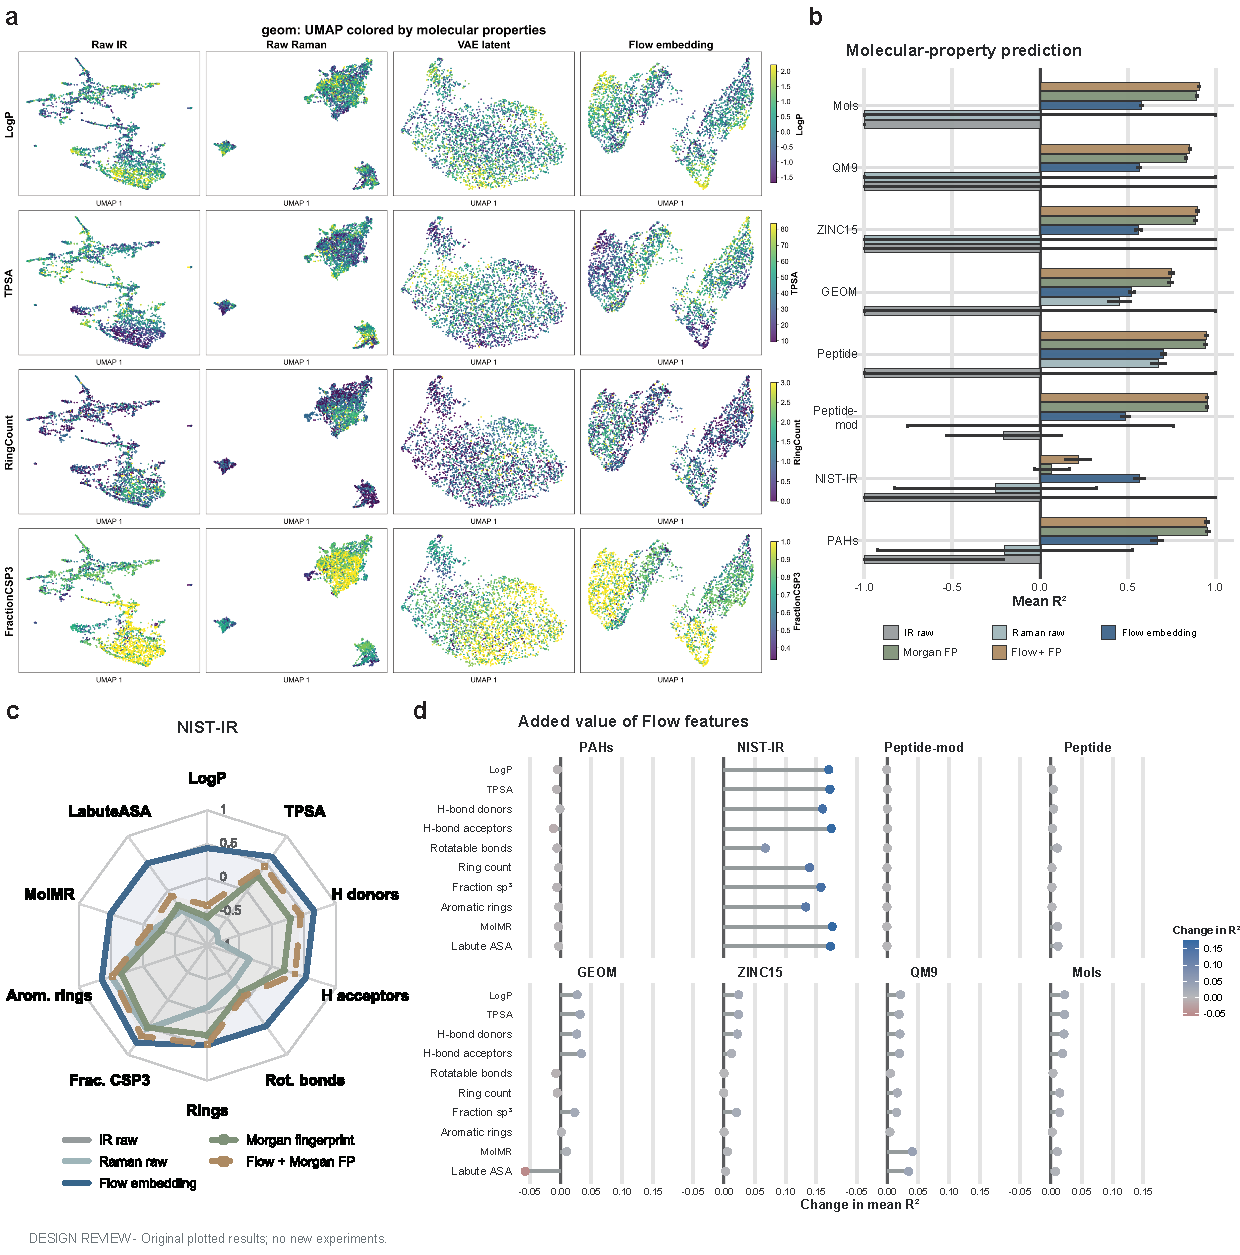
\includegraphics[width=\linewidth]{figs/results/result_3_draw_polished.pdf}
    \caption{\textbf{Molecular information in translation-trained spectral representations.}
\textbf{a,} GEOM UMAP projections of raw IR, raw Raman, VAE latent features and Flow embeddings, coloured by LogP, TPSA, ring count and fraction of sp$^3$ carbons. These projections illustrate representation structure; predictive performance is quantified by regression probes.
\textbf{b,} Mean downstream $R^2$ by dataset for ridge-regression probes using raw IR, raw Raman, Flow embeddings, Morgan fingerprints and concatenated Flow--fingerprint features.
\textbf{c,} Property-wise comparison on NIST-IR. The radar plot compares five feature sets across ten molecular descriptors.
\textbf{d,} Change in mean $R^2$ after adding Flow features to Morgan fingerprints. Positive and negative values indicate improved and reduced probe performance, respectively. Gains vary with property and dataset.}
    \label{fig:quantitative_result_3}
\end{figure}



\section*{Discussion}

\mname\ connects bidirectional spectral translation with molecular representation learning. On the reported computed-spectrum benchmarks, the model improves reconstruction over the evaluated VAE and Transformer baselines. Transfer experiments show lower MAE across the seven held-out ViBench domains, although improvements in $R^2$ are not universal. Frozen embeddings also support molecular-descriptor prediction beyond the original translation task. Together, these observations suggest that learning IR--Raman correspondence can provide both estimates of a missing spectral modality and features useful for downstream analysis.

The contribution of flow matching requires a narrower interpretation than the aggregate benchmark comparison alone permits. SpectraDiT-Direct already achieves strong endpoint accuracy with one network evaluation. The eight-step Flow model performs better in the reported QM9S comparison, but its longer training budget and larger endpoint-loss coefficient prevent attribution of the difference solely to integration. Similarly, the VAE and Transformer comparisons change several architectural and optimization choices at once. The present results support the complete method under the stated protocols; they do not establish that flow integration is necessary for accurate translation or identify the isolated contribution of every loss component.

The learned trajectory offers a way to inspect the mapping between modalities. Intermediate states reveal where intensity changes as the model approaches its prediction, and peak-resolved analyses show that the largest residuals occur near spectral bands. These paths describe numerical transport through spectral space, not vibrational dynamics, reaction pathways or mode-resolved physical mechanisms. Their practical value is diagnostic: they expose the evolution of a prediction and help locate regions where peak position, width or intensity remains inaccurate. Raman$\rightarrow$IR is harder on the three principal benchmarks, but the transfer results show that this directional asymmetry depends on the dataset and metric.

The descriptor probes provide a separate test of representation utility. A frozen nonlinear encoder makes several structure-derived descriptors more accessible to a linear predictor than the raw spectral inputs do. This does not imply that the embedding creates molecular information absent from its source or that it replaces explicit structure. Morgan fingerprints remain a strong reference for descriptors computed from molecular graphs, and combining fingerprints with Flow features helps some tasks while degrading others. Moreover, the probes are fitted separately within each evaluation dataset. The results therefore demonstrate transfer of an encoder, rather than a property predictor that generalizes to a new domain without labelled examples.

Experimental evaluation places further limits on the current model. NIST IR inputs are compared with computed Raman targets, whereas the OpenSpecy/RRUFF study uses a separately trained model and identity-matched spectra from different library records. Neither is a same-specimen, condition-matched experimental benchmark. The modest population-level correlations and the sensitivity to baseline correction show that acquisition conditions and preprocessing remain consequential. The RRUFF development split also overlaps in identifier between optimization and checkpoint selection, and its external test is disjoint by identifier rather than mineral species. These results motivate prospective paired measurements and stricter validation partitions before experimental use.

Several methodological limitations are equally relevant. Sample-wise normalization defines a spectral-shape prediction task; reporting errors after rescaling by target extrema does not demonstrate recovery of unknown absolute intensities. Deterministic integration supplies a point estimate without calibrated uncertainty, particularly problematic when a source spectrum is compatible with multiple target patterns. Molecular overlap across data resources and the provenance of descriptor labels also require explicit accounting when assessing transfer. Future work should prioritize paired experimental data, calibration and uncertainty assessment, together with comparisons that match architectures, optimization budgets and inference cost.

In summary, the reported results support cross-modal spectral translation as a useful objective for normalized spectral completion and molecular feature learning. The next step is to establish how reliably these capabilities extend to calibrated measurements and unfamiliar molecular systems, while resolving the peak-level errors and protocol limitations identified here.


\section*{Online Methods}

\subsection*{Problem setting}

Mathematical notation is summarized in Supplementary Table~\ref{tab:notation}.


Given a source spectrum $x_s\in\mathbb{R}^{L}$ and a target-modality label $m_t\in\{\mathrm{IR},\mathrm{Raman}\}$, the task is to predict the normalized shape of the paired target spectrum $x_t$. Source and target spectra share an ordered wavenumber grid. Batched normalized spectra are denoted by $z_s,z_t\in\mathbb{R}^{B\times L}$. Spectral maps of size $H\times W$ are storage containers, with $L=HW$; they are flattened before entering the one-dimensional SpectraDiT network.

\subsection*{Spectrum preprocessing}

Each source and target spectrum is independently min--max normalized,
\[
\tilde{x}=\frac{x-\min_i x_i}{\max_i x_i-\min_i x_i+\epsilon},
\]
where $\epsilon$ prevents division by zero. The reported benchmark configurations use $L=3600$ for QM9S and QMe14S and $L=1024$ for ViBench. At inference, source normalization requires only the observed source. Target extrema are used for native-scale error reporting, not as model inputs (Appendix~\ref{app:metricdefs}).

\subsection*{Conditional flow matching}

We formulate translation as conditional flow matching~\cite{lipman2023flow,albergo2023building,tong2023conditional}. The model learns a velocity field over spectral states, conditioned on the source spectrum and requested target modality.

For each pair, we sample $\tau\sim\mathcal{U}(0,1)$ independently and construct a linear interpolation~\cite{liu2022rectified,tong2023conditional},
\[
z_\tau=(1-\tau)\,z_s+\tau\,z_t ,
\]
where $z_s$ and $z_t$ are the (batched) source and target spectra. Differentiating this path with respect to $\tau$ gives the ground-truth velocity that the model should reproduce,
\[
u_\tau = \frac{d z_\tau}{d\tau}=z_t-z_s .
\]
A conditional velocity network
\[
v_\theta(z_\tau,\tau,z_s,m_t)\in\mathbb{R}^{B\times L}
\]
is trained to predict $u_\tau$, where $\theta$ denotes its parameters. The architecture supports both directions, with separately trained checkpoints for IR$\rightarrow$Raman and Raman$\rightarrow$IR.

At inference, the target is unavailable. We start from the source and integrate the ordinary differential equation (ODE)~\cite{chen2018neural}
\[
\frac{d z_\tau}{d\tau}
=
v_\theta(z_\tau,\tau,z_s,m_t),
\qquad z_{\tau=0}=z_s ,
\]
from $\tau=0$ to $\tau=1$. The endpoint is the prediction $\hat z_t$. Reported experiments use eight explicit Euler steps. The implementation also supports fourth-order Runge--Kutta integration, which requires four network evaluations per step~\cite{butcher2016numerical}. Integration is deterministic; intermediate states are numerical model states rather than physical vibrational dynamics. Clipping is specified in Appendix~\ref{app:algo}.

\subsection*{Wavenumber-aware SpectraDiT backbone}

SpectraDiT adapts the Diffusion Transformer architecture~\cite{peebles2023scalable} to one-dimensional spectra. Self-attention connects local spectral patches across the wavenumber axis~\cite{vaswani2017attention}.

\paragraph{Tokenization.}
The network input stacks the current transport state $z_\tau$ and the source spectrum $z_s$ as two channels,
\[
[z_\tau,z_s]\in\mathbb{R}^{B\times 2\times L}.
\]
A one-dimensional convolution with kernel size and stride $P$ jointly embeds the two channels into $N=\lceil L/P\rceil$ tokens of width $d$, padding the sequence when necessary. Fixed sinusoidal positional embeddings encode patch location~\cite{vaswani2017attention},
\[
h_0 = \mathrm{PatchEmbed}_{1D}([z_\tau,z_s]) + e_{\mathrm{pos}},
\qquad
h_0\in\mathbb{R}^{B\times N\times d}.
\]

\paragraph{Conditioning.}
The flow time, target modality, and global source-spectrum context are injected through a single conditioning vector
\[
c = W_c\,\operatorname{SiLU}\!\left(e_\tau + e_m + e_s\right)+b_c .
\]
Here $e_\tau$ is a sinusoidal time encoding followed by a multilayer perceptron (MLP), $e_m$ is a learned target-modality embedding, and $e_s$ is a global source summary from a one-dimensional convolutional encoder. The summed embeddings pass through SiLU and an affine projection with parameters $W_c,b_c$.

\paragraph{Transformer blocks.}
Each Transformer block updates the tokens with a multi-head self-attention (MSA) sublayer followed sequentially by an MLP sublayer, both inside residual connections~\cite{vaswani2017attention}. Conditioning is applied through adaptive LayerNorm-Zero (adaLN-Zero), the mechanism introduced for DiT~\cite{peebles2023scalable}: from $c$ we predict per-channel scale/shift parameters that modulate the normalized features ($\mathrm{AdaLN}$), and per-sublayer gates $g_{\mathrm{attn}}(c),g_{\mathrm{mlp}}(c)$ that scale each block's contribution,
\[
\tilde h_\ell
=h_\ell+g_{\mathrm{attn}}(c)\,
\mathrm{MSA}\!\left(\mathrm{AdaLN}_{\mathrm{attn}}(h_\ell,c)\right),
\]
\[
h_{\ell+1}
=\tilde h_\ell+g_{\mathrm{mlp}}(c)\,
\mathrm{MLP}\!\left(\mathrm{AdaLN}_{\mathrm{mlp}}(\tilde h_\ell,c)\right).
\]
The gates are initialized to zero, so each block initially acts as an identity map~\cite{peebles2023scalable}. A final adaptive normalization and linear projection produce length-$P$ velocity patches, which are concatenated and cropped to length $L$.

\subsection*{Spectroscopy-informed spectral objective}

Sparse peaks motivate weighting spectral errors by amplitude and local shape. The objective combines a weighted velocity loss with intermittently evaluated endpoint reconstruction, derivative and local transport terms. These terms encode spectral inductive biases; they do not impose quantum-mechanical selection rules or conservation laws.

\paragraph{Spectral importance weighting.}
Weights are computed from normalized target amplitude $A_i$, absolute first difference $G_i$ and absolute second difference $C_i$:
\[
\begin{aligned}
A_i&=\frac{|z_{t,i}|}{\max_j |z_{t,j}|+\epsilon},\\
G_i&=\frac{|z_{t,i}-z_{t,i-1}|}
{\max_j |z_{t,j}-z_{t,j-1}|+\epsilon},\\
C_i&=\frac{|z_{t,i+1}-2z_{t,i}+z_{t,i-1}|}
{\max_j |z_{t,j+1}-2z_{t,j}+z_{t,j-1}|+\epsilon}.
\end{aligned}
\]
Each cue is normalized by its per-spectrum maximum and combined as
\[
w_i(z_t)
=
1+\alpha_a A_i(z_t)+\alpha_g G_i(z_t)+\alpha_c C_i(z_t),
\]
with $(\alpha_a,\alpha_g,\alpha_c)=(1.0,0.5,0.5)$. The constant term retains non-zero weight outside peaks.

\paragraph{Weighted elastic flow-matching loss.}
The primary training signal asks the predicted velocity to match the ground-truth velocity $u_\tau$. Writing the per-position error
\[
e_i = v_\theta(z_\tau,\tau,z_s,m_t)_i-u_{\tau,i},
\]
we penalize it with an \emph{elastic} (mixed L1/L2) loss, weighted by $w_i$:
\[
\mathcal{L}_{\mathrm{vel}}
=
\frac{1}{BL}
\sum_{b=1}^{B}\sum_{i=1}^{L}
w_{b,i}(z_t)
\left(
\alpha_{\ell_1}|e_{b,i}|
+
(1-\alpha_{\ell_1})e_{b,i}^{2}
\right).
\]
We set $\alpha_{\ell_1}=0.6$. The absolute-error term grows linearly with the residual, whereas the squared-error term gives greater weight to large discrepancies.

\paragraph{Endpoint weighted reconstruction loss.}
To supervise the integrated prediction, we compare $\hat z_t$ with the target using the same weighted elastic criterion,
\[
\mathcal{L}_{\mathrm{end\text{-}elastic}}
=
\frac{1}{BL}
\sum_{b=1}^{B}\sum_{i=1}^{L}
w_{b,i}(z_t)
\left(
\alpha_{\ell_1}|\hat{z}_{t,b,i}-z_{t,b,i}|
+
(1-\alpha_{\ell_1})(\hat{z}_{t,b,i}-z_{t,b,i})^2
\right).
\]
The endpoint prediction is generated by the same eight-step Euler sampler used for evaluation.

\paragraph{Derivative shape loss.}
We penalize differences in first and second finite differences to emphasize peak slopes and curvature,
\[
\mathcal{L}_{\mathrm{shape}}
=
\frac{1}{BL}\sum_{b,i}
\left|
\nabla \hat{z}_{t,b,i}-\nabla z_{t,b,i}
\right|
+
\gamma\,
\frac{1}{BL}\sum_{b,i}
\left|
\nabla^2 \hat{z}_{t,b,i}-\nabla^2 z_{t,b,i}
\right|,
\]
Here $\nabla z_i=z_i-z_{i-1}$ and
$\nabla^2 z_i=z_{i+1}-2z_i+z_{i-1}$.
We use $\gamma=0.5$; the two terms compare local slopes and curvature, respectively.

\paragraph{Local optimal-transport (OT) loss.}
Local optimal transport compares intensity distributions while allowing small peak displacements~\cite{peyre2019computational}. We divide each spectrum into non-overlapping windows $\Omega_k$ of 64 bins, zero-padding the final window if needed, rectify intensities and normalize within each window:
\[
p_i^{(k)}=\frac{\mathrm{ReLU}(\hat{z}_{t,i})+\epsilon}{\sum_{j\in\Omega_k}\left(\mathrm{ReLU}(\hat{z}_{t,j})+\epsilon\right)},
\qquad
q_i^{(k)}=\frac{\mathrm{ReLU}(z_{t,i})+\epsilon}{\sum_{j\in\Omega_k}\left(\mathrm{ReLU}(z_{t,j})+\epsilon\right)},
\]
where $\mathrm{ReLU}(x)=\max(0,x)$. For one-dimensional distributions on an equally spaced grid, the Wasserstein-1 distance is proportional to the absolute difference between cumulative distributions~\cite{peyre2019computational}. Averaging over batches and windows gives
\[
\mathcal{L}_{\mathrm{localOT}}
=
\frac{1}{BK|\Omega|}
\sum_{b=1}^{B}\sum_{k=1}^{K}
\sum_{i\in\Omega_k}
\left|
\sum_{\substack{j\in\Omega_k\\j\le i}}\left(p_{b,j}^{(k)}-q_{b,j}^{(k)}\right)
\right|,
\]
where $K$ is the number of windows and $|\Omega|=64$. The loss is expressed in normalized bin units and restricts transport to each window.

\paragraph{Non-negative intensity prior.}
The implementation includes the one-sided term
\[
\mathcal{L}_{\mathrm{pos}}
=
\frac{1}{BL}
\sum_{b=1}^{B}\sum_{i=1}^{L}
\max(0,-\hat{z}_{t,b,i})^2 .
\]
However, the released sampler clips $\hat z_t$ to $[0,1]$ before evaluating the endpoint losses. Under this implementation, $\mathcal{L}_{\mathrm{pos}}$ is identically zero and contributes no additional training signal. Non-negativity is enforced by output projection; we do not attribute performance gains to this inactive penalty.

\paragraph{Total objective.}
The endpoint-related terms are combined into
\[
\mathcal{L}_{\mathrm{end}}
=
\mathcal{L}_{\mathrm{end\text{-}elastic}}
+
\lambda_{\mathrm{shape}}\mathcal{L}_{\mathrm{shape}}
+
\lambda_{\mathrm{OT}}\mathcal{L}_{\mathrm{localOT}}
+
\lambda_{\mathrm{pos}}\mathcal{L}_{\mathrm{pos}} ,
\]
with $(\lambda_{\mathrm{shape}},\lambda_{\mathrm{OT}},\lambda_{\mathrm{pos}})=(0.05,0.02,0.01)$, retaining the inactive non-negativity term to match the implementation. For each mini-batch, draw $I\sim\mathrm{Bernoulli}(p)$ independently and use
\[
\mathcal{L}_{\mathrm{total}}
=
\mathcal{L}_{\mathrm{vel}}
+
\frac{\lambda_{\mathrm{end}} I}{p}\,
\mathcal{L}_{\mathrm{end}}
\]
with $\lambda_{\mathrm{end}}=0.5$ and $p=0.1$ by default. The rollout is skipped when $I=0$. Since $\mathbb{E}[I/p]=1$, the expected endpoint coefficient is unchanged by $p$; the $p=0.5$ comparison changes its sampling frequency.

\subsection*{Downstream molecular-property probing}

To evaluate whether cross-modal translation produces transferable molecular representations, we extract frozen intermediate features from \mname\ trained on the ViBench-QM9 source domain. For each molecule, the ODE is integrated to flow time $\tau=0.5$, and the final-block SpectraDiT token states are mean-pooled to obtain a fixed-length Flow embedding. The \mname\ parameters remain frozen throughout downstream evaluation.

We evaluate the resulting representations on eight evaluation sets (the QM9 source-domain test set and the seven held-out domains Mols, ZINC15, GEOM, PAHs, NIST-IR, Peptide and Peptide-mod) using ten RDKit molecular descriptors spanning lipophilicity, polarity, hydrogen bonding, flexibility, ring content, saturation, and molecular size. Five feature sets are compared under the same protocol: raw IR spectra, raw Raman spectra, Flow embeddings, 2048-bit radius-2 Morgan fingerprints, and concatenated Flow+Morgan features. Feature standardization is fitted on the training subset of each split, then applied to its test subset. Each representation is evaluated using ridge regression ($\alpha=10$) over five shared random 80/20 train--test splits. $R^2$ is reported as mean $\pm$ standard deviation across the five splits. The same splits are used for all feature sets within each seed to enable paired comparison; UMAP projections are used only for visualization.


\subsection*{Baseline models}

\noindent\textbf{VAE}. We implement a conditional cross-modal variational autoencoder (VAE)~\cite{kingma2014auto} as a reconstruction baseline.
Given $(X_s,m_t)$, the encoder outputs
$\mu,\log \sigma^2\in\mathbb{R}^{B\times d_z}$.
A latent variable $z\in\mathbb{R}^{B\times d_z}$ is sampled via reparameterization,
$z=\mu+\sigma\odot\epsilon$, $\epsilon\sim\mathcal{N}(0,I)$,
and decoded with condition $m_t$ to produce
$\hat{X}_t\in\mathbb{R}^{B\times 1\times H\times W}$.
The reconstruction term is the summed squared error over the batch and all spectral-map positions,
\[
\mathcal{L}_{\mathrm{rec}}
=
\sum_{b,c,h,w}
\left(
\hat{X}_{t,b,c,h,w}-X_{t,b,c,h,w}
\right)^2 .
\]
The KL term is
$D_{\mathrm{KL}}(q_\phi(z|X_s,m_t)\| \mathcal{N}(0,I))$,
and the objective is
$\mathcal{L}_{\mathrm{VAE}}=\mathcal{L}_{\mathrm{rec}}+\beta \mathcal{L}_{\mathrm{KL}}$, where $\beta>0$ is a scalar hyperparameter that balances reconstruction fidelity against the strength of the Gaussian prior regularization.

\noindent\textbf{Transformer}.
We further evaluate a patch-wise Transformer translation baseline. The source spectral map is divided into non-overlapping patches of size $P$ by a stride-$P$ convolution and embedded as a token sequence, with a learnable target-modality embedding added to every token. Six pre-normalized Transformer blocks, each comprising multi-head self-attention and a feed-forward MLP inside residual connections, exchange information globally across all spectral patches. A final layer normalization and linear projection map every token directly to its target patch, after which the patches are reassembled into $\hat{X}_t\in\mathbb{R}^{B\times 1\times H\times W}$ and projected to the normalized intensity range. This provides a deterministic reconstruction comparator with global attention; architecture and optimization differ from SpectraDiT, so the comparison does not isolate flow matching.

\noindent\textbf{SpectraDiT-Direct}.
We construct a QM9S-only Direct comparator using the same velocity-network architecture to contextualize one-pass endpoint prediction. It retains the $22.86$-million-parameter SpectraDiT network, including its source encoder, target-modality conditioning, time embedding, tokenization, and output head, but fixes the flow time to $\tau=0$ and evaluates the network once. The output is interpreted as a residual,
\[
\hat z_t=z_s+f_\theta(z_s,\tau=0,z_s,m_t),
\]
so inference requires one network evaluation (NFE${}=1$) and no ODE solver. Separate models are trained for IR$\rightarrow$Raman and Raman$\rightarrow$IR on the fixed seed-$2$ QM9S split. Both use the same spectral-loss components as \mname; the reported resource-constrained Direct runs use $p=0.1$, $\lambda_{\mathrm{end}}=0.1$, and validation-loss checkpoint selection over $50$ epochs. Because the principal Flow runs use $\lambda_{\mathrm{end}}=0.5$ and a longer optimization budget, this experiment is an architecture-matched one-pass ablation rather than a claim that integration is the only differing training variable.

\subsection*{Implementation details and hyperparameters}

Unless otherwise stated, the QMe14S and ViBench \mname\ models use the configuration in Supplementary Table~\ref{tab:hyperparams}. The released QM9S experiment uses the same SpectraDiT backbone dimensions (hidden width $384$, depth $8$, $6$ attention heads, and patch size $20$) with batch size $32$; its objective weights and eight-step Euler sampler are unchanged.
The endpoint-consistency probability $p$ controls the fraction of mini-batches on which the reconstruction term is evaluated; we use $p=0.1$ by default and additionally evaluate $p=0.5$ in the ablation study (Results).
Models are implemented in PyTorch; the reported benchmark configurations use mixed-precision training on a single GPU.


\subsection*{Data split and reproducibility}

Unless explicitly overridden, paired datasets are split by fixed-seed random partition
(train/validation/test = 0.70/0.15/0.15).
All compared models use identical split indices for fair evaluation. The processed QM9S collection contains $129{,}817$ paired spectra and is partitioned with the fixed seed $2$ into $90{,}871$ training, $19{,}472$ validation, and $19{,}474$ test molecules; the resulting indices are retained and shared across compared models. QMe14S and processed ViBench-Full use their archived fixed-seed partitions shared by all compared models. The separate ViBench transfer experiment instead trains on the curated QM9 source domain and evaluates the supplied QM9 test file and seven held-out domain files in full, without applying another random split. We used four model-initialization seeds for the principal translation experiments while retaining the same data partition within each benchmark.

\subsection*{Experimental-domain evaluation}

\noindent\textbf{NIST--QM9S zero-shot experimental-input domain-shift evaluation.}
Experimental IR spectra were obtained from records associated with the NIST Chemistry WebBook~\citep{nistwebbook}. Because the spectrum files are indexed by PubChem compound identifiers, we retrieved canonical and isomeric SMILES and matched them against the QM9S molecular table after molecular-graph standardization. Matches with identical stereochemistry-aware canonical SMILES were designated \emph{exact}; compounds that agreed only after removal of stereochemical information were designated \emph{connectivity} matches. This procedure yielded 84 unique overlaps (76 exact and 8 connectivity). The NIST spectra contain 3602 intensity samples over approximately $399$--$4000~\mathrm{cm}^{-1}$ in ascending order. We linearly interpolated them onto the 3600-point QM9S grid and applied the same per-spectrum min--max normalization used for model input. No experimental NIST spectrum was used for model fitting or checkpoint selection: the pretrained QM9S IR$\rightarrow$Raman checkpoint was applied directly, and its predictions were compared with computed QM9S Raman spectra for the matched molecules. This evaluates experimental-input/computed-target domain shift. It does not establish that the matched molecular identities are absent from the QM9S training set. Pearson correlation was computed independently for each molecule. For the wavenumber-resolved error profile, we calculated the absolute difference between normalized prediction and target and estimated a 95\% confidence interval of the mean by 1000 molecule-level bootstrap resamples (random seed 42).

\noindent\textbf{OpenSpecy/RRUFF cross-library, identity-matched evaluation.}
IR and Raman records were obtained through an OpenSpecy library snapshot~\citep{cowger2021openspecy} and restricted to records carrying a shared RRUFF identifier~\citep{lafuente2015rruff}. Pairing used the RRUFF identifier rather than a mineral-name string: synonyms were therefore not merged manually, and records with different RRUFF identifiers remained distinct even when they shared the same reported mineral name. The resulting development pool contains 590 RRUFF identifiers (379 mineral names), 595 IR spectra, 1601 Raman spectra, and 4720 constructed within-identifier pairs. The external test set contains 147 pairs from 147 non-overlapping RRUFF identifiers and 135 mineral names; a mineral name can therefore occur more than once, but no RRUFF identifier contributes more than one test pair. Seventy-two of the 135 test mineral names also occur under different RRUFF identifiers in the development pool, so this is RRUFF-ID-disjoint rather than mineral-species-disjoint evaluation. Most importantly, cross-library identity matching does not imply that an IR spectrum and Raman spectrum were measured from the same specimen or under matched composition, polymorph purity, orientation, instrument, or environmental conditions.

The 4720 development pairs were split with random seed 42 into 3304 optimization pairs (70\%), 708 checkpoint-selection pairs (15\%), and 708 unused internal pairs (15\%). This internal split was performed at the constructed-pair level, so its RRUFF identifiers overlap; only the external test identifiers are disjoint from the full development pool. Supplementary Table~\ref{tab:rruff-split} reports both RRUFF identifiers and mineral names to distinguish records from species.


All spectra were interpolated to 576 points and min--max normalized per spectrum; no baseline correction was applied during model training. Every materialized pair row was sampled through a shuffled data loader, so an IR or Raman record could participate in multiple development pairs when several records shared its RRUFF identifier. The experimental-domain model used the one-dimensional SpectraDiT backbone with hidden width 384, eight Transformer blocks, six attention heads, patch size 4, batch size 32, Adam learning rate $2\times10^{-4}$, cosine annealing, and the fixed reproducibility seed 42. It was trained for 30 epochs, and the checkpoint with the lowest generation loss on the 708-pair checkpoint-selection subset was retained. At evaluation, Pearson correlation was calculated after restoring physical wavenumber order. To assess sensitivity to broad backgrounds, we additionally applied asymmetric least-squares baseline correction independently to every predicted and reference Raman spectrum, using a smoothness parameter of $10^5$, asymmetry parameter $0.01$, and 10 iterations, and recomputed Pearson correlation. Representative overlays in Fig.~\ref{fig:experimental_validation} were selected from test samples with raw $\text{R}^2>0.5$ and ranked by raw Pearson correlation while retaining at most one example per reported mineral name; the accompanying full distributions provide population-level context.

\paragraph{Statistical analysis.} Principal translation experiments are repeated over four model-initialization seeds using fixed test partitions. Comparisons between SpectraFlow and the strongest baseline use paired molecule-level metric values on the shared test set and a two-sided Wilcoxon signed-rank test. P-values across dataset–direction comparisons are adjusted using the Holm–Bonferroni procedure, with adjusted p$<$0.05 considered statistically significant.


\section*{Declarations}

\bmhead{Data availability}
All datasets used in this study are publicly accessible from their cited sources. QM9S is available through its original release~\citep{zou2023deep}, ViBench accompanies Vib2Mol~\citep{lu2025vib2mol}, and QMe14S is released by \citet{yuan2025qme14s}. The experimental-input analysis uses IR records associated with the NIST Chemistry WebBook (SRD 69; DOI: \texttt{10.18434/T4D303})~\citep{nistwebbook}. The cross-library analysis uses an OpenSpecy snapshot and records carrying RRUFF identifiers~\citep{cowger2021openspecy,lafuente2015rruff}; source resources were last accessed on 14 July 2026. OpenSpecy software is distributed under CC BY 4.0, while contributed spectra can carry record-specific Creative Commons terms; NIST SRD and RRUFF records remain subject to their respective source terms. To preserve those terms, the released repository provides identifiers, pairing manifests, preprocessing code, and split assignments rather than relicensing third-party spectra. No new raw spectral data were generated.

\bmhead{Code availability}
Model definitions, training and evaluation scripts, and downstream-analysis code are available at \url{https://github.com/jiaqingxie/SpectraFlow}.

\bmhead{Competing interests}
The authors declare no competing interests.

\bmhead{Author contributions}
J.X. developed the method, implemented the experiments and analyses, and prepared the initial manuscript. All authors contributed to the conception of the study, interpretation of the results, and critical revision of the manuscript. All authors read and approved the final version.

\bmhead{Funding}
Tianfan Fu is supported by the Young Scientists Fund (C Class) of the National Natural Science Foundation of China (Grant No.~62506154), the Fundamental Research Funds for the Central Universities and the Nanjing University International Collaboration Initiative (Grant No.~020214380129), and the ``111 Center'' (No.~B26023).

\begin{appendices}
\renewcommand{\thefigure}{S\arabic{figure}}
\renewcommand{\thetable}{S\arabic{table}}
\renewcommand{\theHfigure}{supp.\arabic{figure}}
\renewcommand{\theHtable}{supp.\arabic{table}}
\setcounter{figure}{0}
\setcounter{table}{0}

\section{Supporting methods and benchmark comparisons}\label{app:supporting-tables}
The following tables provide notation, model settings, the one-pass comparison, transfer results and cross-library split composition. Numerical entries are those used in the main analyses. The Direct comparison uses different training budgets and is not an integration-only ablation.

\begin{table}[htbp]
\centering
\caption{\textbf{Summary of mathematical notation.}}
\label{tab:notation}
\begin{tabular}{@{}ll@{}}
\toprule
Symbol & Meaning \\
\midrule
$x_s,\,x_t\in\mathbb{R}^{L}$ & source / target spectrum (length $L$) \\
$m_s,\,m_t$ & source / target modality label ($\mathrm{IR}$ or $\mathrm{Raman}$) \\
$X_s,\,X_t\in\mathbb{R}^{1\times H\times W}$ & spectral map (heatmap) form of a spectrum \\
$z_s,\,z_t\in\mathbb{R}^{B\times L}$ & flattened source / target sequences in a batch \\
$\tau\in[0,1]$ & flow (transport) time \\
$z_\tau$ & intermediate transport state at time $\tau$ \\
$u_\tau$ & ground-truth velocity along the probability path \\
$v_\theta$ & learnable conditional velocity network (\mname-DiT) \\
$\hat{z}_t$ & predicted target spectrum (ODE endpoint) \\
$B,\,L$ & batch size, spectral sequence length \\
$N,\,P,\,d$ & number of tokens, patch size, hidden width \\
$e_{\mathrm{pos}},\,e_\tau,\,e_m,\,e_s$ & position / time / modality / source embeddings \\
$c$ & fused conditioning vector \\
$h_\ell$ & token features at Transformer block $\ell$ \\
$A_i,\,G_i,\,C_i$ & normalized amplitude / gradient / curvature at $i$ \\
$w_i$ & spectral importance weight at position $i$ \\
$\alpha_a,\alpha_g,\alpha_c$ & weights for amplitude / gradient / curvature \\
$\alpha_{\ell_1}$ & L1-vs-L2 mixing coefficient of the elastic loss \\
$\nabla,\,\nabla^2$ & discrete first / second derivative operators \\
$\Omega_k,\,K$ & $k$-th local window and number of windows \\
$p_i^{(k)},\,q_i^{(k)}$ & normalized predicted / target intensity in $\Omega_k$ \\
$\lambda_{\mathrm{shape}},\lambda_{\mathrm{OT}},\lambda_{\mathrm{pos}}$ & weights of shape / OT / non-negativity terms \\
$\gamma$ & curvature weight inside the shape loss \\
$\lambda_{\mathrm{end}},\,p$ & endpoint-loss weight and its application probability \\
$\beta,\,d_z$ & VAE KL weight and latent dimension (baseline) \\
$\epsilon$ & small constant for numerical stability \\
\bottomrule
\end{tabular}
\end{table}

\begin{table}[htbp]
\centering
\caption{\textbf{Default QMe14S/ViBench hyperparameters of \mname.} The QM9S configuration is specified in the accompanying text. The non-negativity coefficient is retained for implementation consistency, but its penalty is zero after output clipping.}
\label{tab:hyperparams}
\begin{tabular}{@{}lll@{}}
\toprule
Group & Hyperparameter & Value \\
\midrule
\multirow{8}{*}{Architecture}
 & Input channels $[z_\tau,z_s]$ & $2$ \\
 & Hidden width $d$ & $384$ \\
 & DiT blocks (depth) & $8$ \\
 & Attention heads & $6$ \\
 & MLP ratio & $4.0$ \\
 & Patch size $P$ & $20$ \\
 & Positional embedding & fixed 1D sinusoidal \\
 & Conditioning & adaLN-Zero \\
\midrule
\multirow{7}{*}{Optimization}
 & Optimizer & Adam \\
 & Learning rate & $2\times10^{-4}$ \\
 & Weight decay & $0$ \\
 & LR schedule & cosine annealing \\
 & Batch size & $64$ \\
 & Gradient clipping & $1.0$ \\
 & Epochs & $100$ \\
\midrule
\multirow{8}{*}{Objective}
 & Elastic mix $\alpha_{\ell_1}$ & $0.6$ \\
 & Amplitude / grad. / curv. $(\alpha_a,\alpha_g,\alpha_c)$ & $(1.0,\,0.5,\,0.5)$ \\
 & Endpoint weight $\lambda_{\mathrm{end}}$ & $0.5$ \\
 & Shape weight $\lambda_{\mathrm{shape}}$ & $0.05$ \\
 & Local-OT weight $\lambda_{\mathrm{OT}}$ & $0.02$ \\
 & Nonneg. weight $\lambda_{\mathrm{pos}}$ & $0.01$ \\
 & Endpoint probability $p$ & $0.1$ \\
 & Local-OT window & $64$ points \\
\midrule
\multirow{3}{*}{Sampling}
 & Train-time endpoint ODE steps & $8$ \\
 & Inference ODE steps & $8$ \\
 & ODE solver & Euler / RK4 \\
\bottomrule
\end{tabular}
\end{table}

\begin{table}[htbp]
\centering
\caption{\textbf{One-pass SpectraDiT-Direct ablation on QM9S.} Direct retains the full $22.86$-million-parameter SpectraDiT velocity-network architecture but predicts the endpoint residual with one network evaluation and no ODE integration. Direct values are from the fixed seed-$2$ run and are rounded to three decimals; the corresponding eight-step Euler \mname\ values are reproduced from Table~\ref{tab:reconstruction} for context. Because the Direct run used a shorter optimization budget and a lower endpoint-loss coefficient (Methods), this is an architecture-matched one-pass ablation rather than a strict integration-only comparison.}
\label{tab:direct-ablation}
\begin{tabular}{llcc}
\toprule
Direction & Model & $\text{R}^2\uparrow$ & Pearson $r\uparrow$ \\
\midrule
\multirow{2}{*}{IR$\rightarrow$Raman}
& SpectraDiT-Direct (NFE${}=1$) & $0.910$ & $0.960$ \\
& \mname\ (NFE${}=8$) & $\mathbf{0.939}$ & $\mathbf{0.976}$ \\
\midrule
\multirow{2}{*}{Raman$\rightarrow$IR}
& SpectraDiT-Direct (NFE${}=1$) & $0.806$ & $0.913$ \\
& \mname\ (NFE${}=8$) & $\mathbf{0.830}$ & $\mathbf{0.926}$ \\
\bottomrule
\end{tabular}
\end{table}

\begin{table*}[t]
\centering
\small
\caption{Generalization comparison of VAE and \mname\ across ViBench benchmark datasets. Models are trained on ViBench-QM9 and evaluated on its test set and seven held-out domains. Values are reported as VAE / \mname\ (mean $\pm$ s.d.); the better value is shown in bold. MAE is reported in units of $10^{-2}$; lower MAE and higher $\text{R}^2$ indicate better performance.}
\label{tab:vae-vibraflow-main}
\resizebox{\textwidth}{!}{%
\begin{tabular}{lcccc}
\toprule
Dataset & \multicolumn{2}{c}{IR$\to$Raman} & \multicolumn{2}{c}{Raman$\to$IR} \\
\cmidrule(lr){2-3}\cmidrule(lr){4-5}
 & MAE ($\downarrow, \times 10^{-2}$) & $\text{R}^2 (\uparrow)$ & MAE ($\downarrow, \times 10^{-2}$) & $\text{R}^2 (\uparrow)$ \\
\midrule
QM9 & 1.53 $\pm$ 0.02 / \textbf{1.16 $\pm$ 0.01} & 0.780 $\pm$ 0.004 / \textbf{0.835 $\pm$ 0.004} & 1.61 $\pm$ 0.01 / \textbf{1.32 $\pm$ 0.01} & 0.657 $\pm$ 0.002 / \textbf{0.708 $\pm$ 0.001} \\
Mols & 1.43 $\pm$ 0.02 / \textbf{1.22 $\pm$ 0.01} & 0.778 $\pm$ 0.001 / \textbf{0.789 $\pm$ 0.001} & 1.36 $\pm$ 0.02 / \textbf{1.35 $\pm$ 0.03} & \textbf{0.718 $\pm$ 0.004} / 0.675 $\pm$ 0.010 \\
PAHs & 2.78 $\pm$ 0.03 / \textbf{2.62 $\pm$ 0.03} & -0.170 $\pm$ 0.009 / \textbf{-0.155 $\pm$ 0.019} & 2.63 $\pm$ 0.02 / \textbf{2.53 $\pm$ 0.01} & \textbf{0.221 $\pm$ 0.011} / 0.193 $\pm$ 0.015 \\
ZINC15 & 2.35 $\pm$ 0.01 / \textbf{2.09 $\pm$ 0.02} & 0.470 $\pm$ 0.003 / \textbf{0.503 $\pm$ 0.006} & 2.14 $\pm$ 0.02 / \textbf{1.98 $\pm$ 0.00} & 0.371 $\pm$ 0.006 / \textbf{0.380 $\pm$ 0.004} \\
GEOM & 1.45 $\pm$ 0.02 / \textbf{1.10 $\pm$ 0.01} & 0.811 $\pm$ 0.002 / \textbf{0.859 $\pm$ 0.002} & 1.80 $\pm$ 0.01 / \textbf{1.50 $\pm$ 0.01} & 0.626 $\pm$ 0.003 / \textbf{0.678 $\pm$ 0.003} \\
Peptide & 3.61 $\pm$ 0.04 / \textbf{3.48 $\pm$ 0.05} & 0.529 $\pm$ 0.011 / \textbf{0.532 $\pm$ 0.022} & 3.35 $\pm$ 0.03 / \textbf{3.22 $\pm$ 0.04} & 0.106 $\pm$ 0.008 / \textbf{0.135 $\pm$ 0.003} \\
Peptide-mod & 4.13 $\pm$ 0.05 / \textbf{4.02 $\pm$ 0.01} & \textbf{0.430 $\pm$ 0.018} / 0.416 $\pm$ 0.006 & 3.62 $\pm$ 0.02 / \textbf{3.52 $\pm$ 0.04} & 0.012 $\pm$ 0.006 / \textbf{0.030 $\pm$ 0.011} \\
NIST-IR & 2.14 $\pm$ 0.01 / \textbf{1.90 $\pm$ 0.01} & 0.467 $\pm$ 0.003 / \textbf{0.495 $\pm$ 0.002} & 2.08 $\pm$ 0.01 / \textbf{1.94 $\pm$ 0.02} & 0.365 $\pm$ 0.004 / \textbf{0.367 $\pm$ 0.010} \\
\bottomrule
\end{tabular}%
}
\end{table*}

\begin{table*}[htbp]
\centering
\caption{\textbf{Composition of the OpenSpecy/RRUFF cross-library evaluation.} Counts of RRUFF identifiers and mineral names are both reported because multiple RRUFF records can share a mineral name. Optimization and checkpoint-selection rows are pair-level subsets of the same development pool and therefore overlap in identity; the external test set is disjoint by RRUFF identifier.  }
\label{tab:rruff-split}
\scriptsize
\setlength{\tabcolsep}{6pt}
\begin{tabular}{lccccc}
\toprule
Split & RRUFF & Mineral & IR & Raman & Constructed pairs \\
\midrule
Optimization & 590 & 379 & 595 & 1512 & 3304 \\
Checkpoint selection & 421 & 289 & 421 & 601 & 708 \\
Unused internal remainder & 419 & 301 & 420 & 592 & 708 \\
External test & 147 & 135 & 147 & 147 & 147 \\
\bottomrule
\end{tabular}
\end{table*}


\section{Dataset details and statistics}\label{app:data}

We train and evaluate \mname\ on three paired infrared--Raman benchmarks---QM9S, QMe14S, and ViBench~\citep{lu2025vib2mol,yuan2025qme14s}---whose overall composition is summarized in Supplementary Fig.~\ref{fig:dataset_stats}. Each ``sample'' is a molecule associated with paired IR and Raman spectra. The in-distribution experiments use fixed-seed partitions shared by all compared models. The ViBench transfer protocol is separate: it trains on the curated QM9 source domain and evaluates the supplied domain-specific test files without repartitioning them.

\begin{figure}[htbp]
    \centering
    \begin{minipage}{\linewidth}\centering
        {\footnotesize\textbf{(a)}}\\[1pt]
        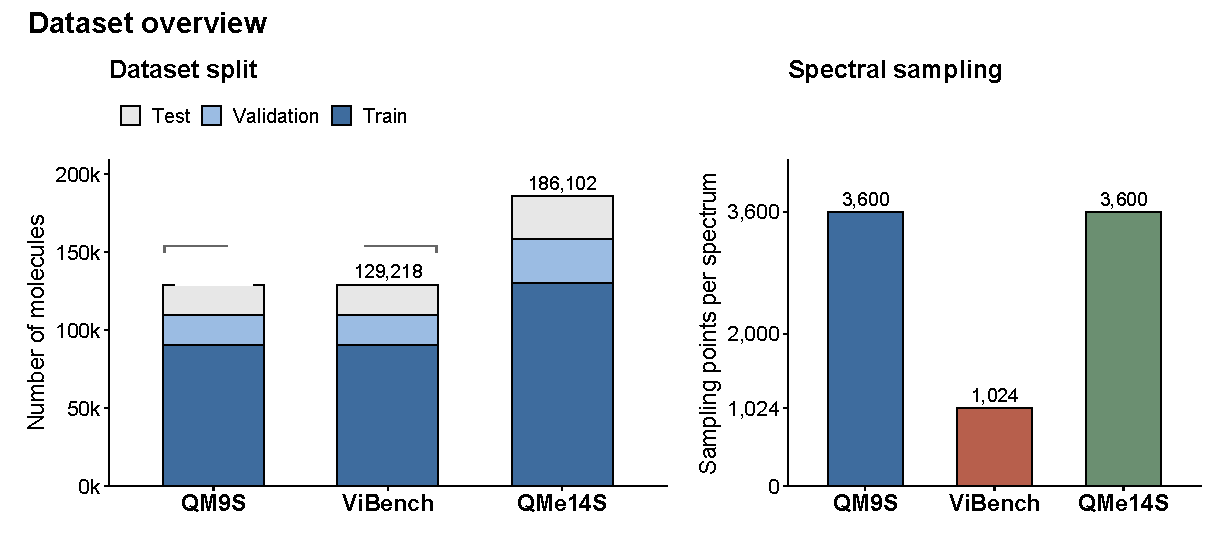
\includegraphics[width=0.96\linewidth]{figs/dataset_overview.pdf}
    \end{minipage}\\[10pt]
    \begin{minipage}{\linewidth}\centering
        {\footnotesize\textbf{(b)}}\\[1pt]
        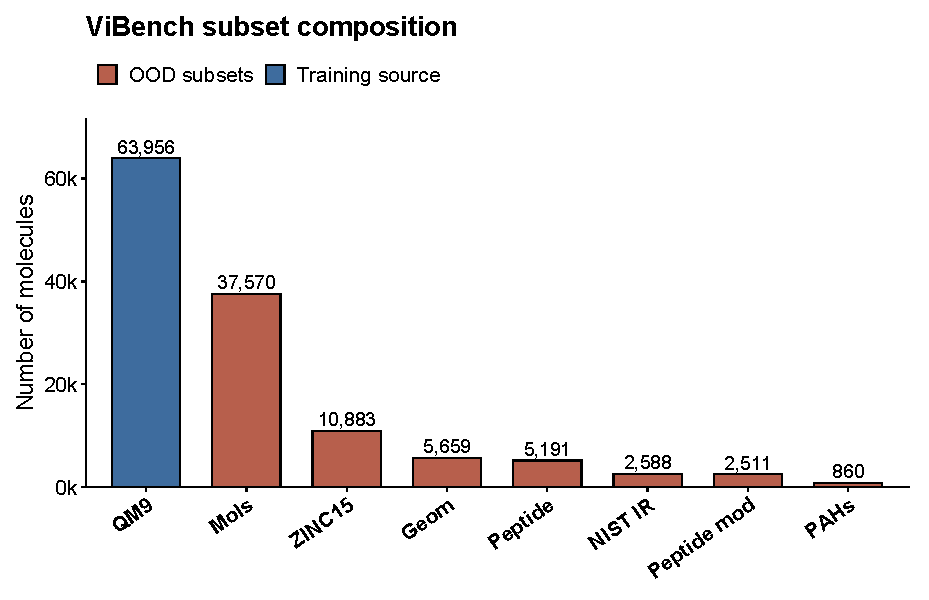
\includegraphics[width=0.66\linewidth]{figs/vibench_subset_distribution.pdf}
    \end{minipage}
    \caption{\textbf{Dataset composition and statistics.}
    \textbf{a)} Overview of the three benchmarks. Left: number of entries per dataset, decomposed into the fixed train/validation/test split; QM9S contains $129{,}817$ entries, ViBench contains $129{,}218$ entries, and QMe14S is a larger and chemically more diverse collection of $186{,}102$ molecules. Right: number of sampling points per spectrum (spectral length $L$); QM9S and QMe14S use $L{=}3600$, while ViBench uses $L{=}1024$.
    \textbf{b)} Composition of ViBench by sub-domain. ViBench is partitioned into the in-distribution QM9 training source ($63{,}956$ molecules, $49.5\%$; blue) and seven held-out out-of-distribution (OOD) evaluation subsets (red): Mols ($37{,}570$; $29.1\%$), ZINC15 ($10{,}883$; $8.4\%$), GEOM ($5{,}659$; $4.4\%$), Peptide ($5{,}191$; $4.0\%$), NIST-IR ($2{,}588$; $2.0\%$), Peptide-mod ($2{,}511$; $1.9\%$), and PAHs ($860$; $0.7\%$). Percentages are relative to the full ViBench ($129{,}218$ molecules). The OOD subset sizes equal the number of paired test spectra used for the cross-dataset generalization experiments in the main text.}
    \label{fig:dataset_stats}
\end{figure}

\paragraph{QM9S.} The processed QM9S collection used here provides computed IR and Raman spectra for $129{,}817$ small organic molecules drawn from the QM9 chemical space (up to nine heavy atoms, C/N/O/F). Each spectrum is sampled at $L{=}3600$ wavenumber points and reshaped into a $60\times60$ single-channel spectral map for the data pipeline; the fixed split contains $90{,}871$ training, $19{,}472$ validation, and $19{,}474$ paired test molecules. QM9S serves as our primary in-distribution benchmark for both IR$\rightarrow$Raman and Raman$\rightarrow$IR translation.

\paragraph{QMe14S.} QMe14S~\citep{yuan2025qme14s} is a substantially larger and chemically broader benchmark of $186{,}102$ molecules with the same full-resolution sampling ($L{=}3600$, $60\times60$ maps), giving $27{,}916$ paired test molecules. Its wider elemental and structural coverage makes it a more demanding in-distribution test of translation fidelity, and the larger absolute spectral intensities are reflected in the correspondingly larger RMSE scale reported for QMe14S in the main text.

\paragraph{ViBench.} ViBench~\citep{lu2025vib2mol} is a distinct multi-domain vibrational benchmark whose entries total $129{,}218$ and whose spectra are represented at $L{=}1024$ points ($32\times32$ maps). Its QM9 source domain and seven chemically distinct evaluation domains are not a compressed copy of the QM9S molecular collection. We use the processed ViBench collection in two ways. \emph{ViBench-Full} denotes the in-distribution split used in Table~\ref{tab:reconstruction} ($13{,}793$ paired test molecules). For the out-of-distribution study, we follow the curated ViBench-QM9 protocol of Vib2Mol~\citep{lu2025vib2mol}: \mname\ is trained \emph{only} on the QM9 source domain and then evaluated, without any per-dataset tuning, on its own QM9 test split and on seven held-out domains that span markedly different chemistries (Supplementary Fig.~\ref{fig:dataset_stats}b).

\paragraph{Out-of-distribution evaluation subsets.} The seven held-out ViBench domains are designed to probe transfer to chemistries that are absent from, or under-represented in, the QM9 training source. \emph{Mols} ($37{,}570$) collects general organic molecules; \emph{ZINC15} ($10{,}883$) consists of drug-like molecules sampled from the ZINC15 library; \emph{GEOM} ($5{,}659$) is drawn from the GEOM conformer collection; \emph{Peptide} ($5{,}191$) and \emph{Peptide-mod} ($2{,}511$) comprise (chemically modified) peptides whose repeated backbone motifs and large sizes differ strongly from QM9; \emph{NIST-IR} ($2{,}588$) contains molecules associated with experimental NIST infrared references; and \emph{PAHs} ($860$) gathers polycyclic aromatic hydrocarbons dominated by extended conjugated ring systems. For each subset, the reported count is the number of paired spectra in the supplied domain test file; each file is evaluated in full, with no additional $70/15/15$ split. These supplied files are used to compute the cross-dataset MAE and $\text{R}^2$ values in Supplementary Table~\ref{tab:vae-vibraflow-main} and Fig.~\ref{fig:quantitative_result}b--c.

\paragraph{Preprocessing.} Across all datasets, every spectrum is min--max normalized per sample (Methods) before being flattened to the one-dimensional wavenumber sequence consumed by \mname; QM9S and QMe14S use $L{=}3600$ and ViBench uses $L{=}1024$. No per-dataset retuning is applied: the backbone width, depth, and number of heads are fixed across datasets, and only the sequence length $L$ (and hence the token count $N{=}\lceil L/P\rceil$) varies with the spectral map size.

\section{Training and inference algorithms}\label{app:algo}

The algorithms summarize the conditional flow-matching objective and deterministic sampler; all symbols follow Supplementary Table~\ref{tab:notation}, and the default hyperparameter values are those of Supplementary Table~\ref{tab:hyperparams}.

\subsection{Training}
Algorithm~\ref{alg:train} summarizes one training epoch. Each mini-batch contains paired source/target spectra $(z_s,z_t)$ together with the target-modality label $m_t$ (with $m_t{=}2$ for a Raman target and $m_t{=}0$ for an IR target in the implementation's IR/UV/Raman index map). We train separate direction-specific checkpoints, reversing the source and target spectra for the Raman$\rightarrow$IR experiment. For every sample we draw an independent flow time $\tau\sim\mathcal{U}(0,1)$, form the straight-line interpolation $z_\tau=(1-\tau)z_s+\tau z_t$, and take the constant displacement $u_\tau=z_t-z_s$ as the ground-truth velocity. The network prediction $v_\theta(z_\tau,\tau,z_s,m_t)$ is matched to $u_\tau$ with the weighted elastic loss $\mathcal{L}_{\mathrm{vel}}$, using the target-derived spectral importance weight $w(z_t)=1+\alpha_a A+\alpha_g G+\alpha_c C$ that up-weights peaks, edges, and sharp features.

The endpoint-consistency term is evaluated stochastically because integrating the ODE during training is expensive: with probability $p$ we roll out the sampler for $N_{\mathrm{tr}}$ steps to obtain $\hat z_t$, and accumulate the endpoint elastic, derivative-shape, local-OT, and non-negativity penalties into $\mathcal{L}_{\mathrm{end}}$. Dividing $\mathcal{L}_{\mathrm{end}}$ by $p$ makes its expected contribution equal to applying it on every batch, so the velocity term defines the primary flow-matching objective, while the spectroscopy-informed endpoint terms provide auxiliary supervision.  Parameters are updated with Adam under gradient clipping, and a cosine schedule decays the learning rate over the run; the checkpoint with the lowest normalized validation endpoint reconstruction loss (the elastic L1/L2 criterion) is retained.

\begin{algorithm}[!htb]
\small
\caption{\mname\ training (one epoch)}\label{alg:train}
\begin{algorithmic}[1]
\Require paired spectra $\{(z_s,z_t,m_t)\}$; velocity net $v_\theta$; weights $\alpha_a,\alpha_g,\alpha_c,\alpha_{\ell_1}$; loss weights $\lambda_{\mathrm{end}},\lambda_{\mathrm{shape}},\lambda_{\mathrm{OT}},\lambda_{\mathrm{pos}}$; endpoint probability $p$; train-time ODE steps $N_{\mathrm{tr}}$; solver $\in\{\text{Euler},\text{RK4}\}$
\For{each mini-batch $(z_s,z_t,m_t)$}
  \State $\tau \sim \mathcal{U}(0,1)$ \Comment{independent per-sample flow time}
  \State $z_\tau \gets (1-\tau)\,z_s + \tau\,z_t$ \Comment{straight-line interpolation}
  \State $u_\tau \gets z_t - z_s$ \Comment{ground-truth constant velocity}
  \State $w \gets 1+\alpha_a A(z_t)+\alpha_g G(z_t)+\alpha_c C(z_t)$ \Comment{importance weight}
  \State $\hat u \gets v_\theta(z_\tau,\tau,z_s,m_t)$
  \State $\mathcal{L}_{\mathrm{vel}} \gets$ weighted elastic loss between $\hat u$ and $u_\tau$ with weight $w$
  \State $\mathcal{L}_{\mathrm{end}} \gets 0$
  \If{$\lambda_{\mathrm{end}}>0$ \textbf{and} $\mathrm{Bernoulli}(p)=1$}
     \State $\hat z_t \gets \Call{ODESample}{v_\theta,z_s,m_t,N_{\mathrm{tr}},\text{solver}}$
     \State $\mathcal{L}_{\mathrm{end}} \gets \mathcal{L}_{\mathrm{end\text{-}elastic}}(\hat z_t,z_t;w) + \lambda_{\mathrm{shape}}\mathcal{L}_{\mathrm{shape}} + \lambda_{\mathrm{OT}}\mathcal{L}_{\mathrm{localOT}} + \lambda_{\mathrm{pos}}\mathcal{L}_{\mathrm{pos}}$
  \EndIf
  \State $\mathcal{L} \gets \mathcal{L}_{\mathrm{vel}} + \dfrac{\lambda_{\mathrm{end}}}{p}\,\mathcal{L}_{\mathrm{end}}$
  \State $\theta \gets \mathrm{Adam\text{-}update}\big(\theta,\nabla_\theta\mathcal{L}\big)$ \Comment{gradient clipping at $1.0$}
\EndFor
\end{algorithmic}
\end{algorithm}

\subsection{Inference}
At inference the target spectrum is unknown, so we reconstruct it by integrating the learned velocity field from the source. Algorithm~\ref{alg:sample} details the deterministic ODE sampler used both at test time and inside the endpoint term during training. Starting from $z{=}z_s$ with a uniform step $\Delta\tau=1/N$, we advance from $\tau{=}0$ to $\tau{=}1$ using either the explicit Euler update (one network evaluation per step) or the fourth-order Runge--Kutta update (four evaluations per step, higher accuracy at greater cost). For numerical stability, every evaluated velocity is clipped to $[-2,2]$, intermediate states before the final step are clipped to $[-0.1,1.1]$, and the endpoint is projected to the normalized intensity interval $[0,1]$. Because the dynamics are deterministic and conditioned only on $(z_s,m_t)$, a given source always yields the same prediction and every intermediate state $z_\tau$ is inspectable. The reported translation experiments use $N{=}8$ Euler steps, and the in-training endpoint rollout likewise uses $N_{\mathrm{tr}}{=}8$ Euler steps.

\begin{algorithm}[!htb]
\small
\caption{\textsc{ODESample}: deterministic flow integration}\label{alg:sample}
\begin{algorithmic}[1]
\Require trained $v_\theta$; source spectrum $z_s$; target modality $m_t$; steps $N$; solver $\in\{\text{Euler},\text{RK4}\}$
\State $z \gets z_s$;\quad $\Delta\tau \gets 1/N$
\State Define $\bar v_\theta(\cdot)\gets\operatorname{clip}(v_\theta(\cdot),-2,2)$
\For{$i=0,1,\dots,N-1$}
  \State $\tau_0 \gets i\,\Delta\tau$
  \If{solver $=$ Euler}
     \State $z \gets z + \Delta\tau\; \bar v_\theta(z,\tau_0,z_s,m_t)$
  \Else \Comment{RK4}
     \State $k_1 \gets \bar v_\theta(z,\;\tau_0,\;z_s,m_t)$
     \State $k_2 \gets \bar v_\theta\big(z+\tfrac12\Delta\tau\,k_1,\;\tau_0+\tfrac12\Delta\tau,\;z_s,m_t\big)$
     \State $k_3 \gets \bar v_\theta\big(z+\tfrac12\Delta\tau\,k_2,\;\tau_0+\tfrac12\Delta\tau,\;z_s,m_t\big)$
     \State $k_4 \gets \bar v_\theta\big(z+\Delta\tau\,k_3,\;\tau_0+\Delta\tau,\;z_s,m_t\big)$
     \State $z \gets z + \tfrac{\Delta\tau}{6}\big(k_1+2k_2+2k_3+k_4\big)$
  \EndIf
  \If{$i<N-1$}
     \State $z\gets\operatorname{clip}(z,-0.1,1.1)$
  \EndIf
\EndFor
\State $\hat z_t \gets \operatorname{clip}(z,0,1)$ \Comment{normalized-intensity projection}
\State \Return $\hat z_t$
\end{algorithmic}
\end{algorithm}

\section{Illustrative Raman-computation timing}\label{app:raman-timing}

To obtain an order-of-magnitude estimate of the computational opportunity, we performed a small local timing probe with the GFN2-xTB~\citep{bannwarth2019gfn2} Hessian and PTB~\citep{grimme2023ptb} polarizability-derivative implementation distributed with MLatom~3.23.4~\citep{dral2024mlatom} (xTB~6.7.0). Calculations used four CPU threads on an Intel Core Ultra~9~275HX and fixed input geometries; geometry optimization was excluded. For each molecule, the IR-only command evaluated the Hessian, whereas the Raman command additionally evaluated PTB polarizability derivatives. Supplementary Table~\ref{tab:raman-timing} reports the median wall time over five repetitions. The additional Raman-response cost increased from $0.040$\,s for methane to $1.233$\,s for ethylbenzene. This three-molecule probe is intended only as a computational scale estimate, not as a comprehensive quantum-chemical timing benchmark; the benchmark script is released with the code (Code availability).

\begin{table*}[htbp]
\centering
\caption{\textbf{Illustrative GFN2-xTB/PTB timing probe.} Values are median wall times over five runs with four CPU threads. ``Additional Raman'' is the difference between the joint Hessian/polarizability-derivative calculation and the Hessian-only calculation; geometry optimization is not included.}
\label{tab:raman-timing}
\begin{tabular}{lrrrr}
\toprule
Molecule & Atoms & IR-only (s) & IR+Raman (s) & Additional Raman (s) \\
\midrule
Methane      & 5  & 0.103 & 0.143 & 0.040 \\
Ethanol      & 9  & 0.148 & 0.261 & 0.113 \\
Ethylbenzene & 18 & 0.276 & 1.509 & 1.233 \\
\bottomrule
\end{tabular}
\end{table*}

\section{Evaluation metric definitions}\label{app:metricdefs}

Before evaluation, each normalized prediction is mapped back with the minimum and maximum of its paired target spectrum. These target statistics are used only to report errors on the native intensity scale and are not inputs to the translation network; in a deployment setting where the target modality is absent, the model predicts the normalized spectral shape unless an external intensity calibration is available. Unless a normalized analysis is explicitly specified, translation metrics are computed per test molecule from the reference spectrum $y\in\mathbb{R}^{L}$ and prediction $\hat y\in\mathbb{R}^{L}$ and averaged over the test set; translation results are summarized over four model-initialization seeds, whereas downstream probing results are summarized over five shared random train/test splits.


Consequently, absolute-error metrics such as MAE and RMSE are dataset-scale dependent, whereas $\text{R}^2$ and Pearson correlation are unchanged by applying the same affine rescaling to the reference and prediction. We write $\bar y=\tfrac1L\sum_i y_i$, $\bar{\hat y}=\tfrac1L\sum_i \hat y_i$, and $\mathrm{MSE}=\tfrac1L\sum_{i=1}^{L}(y_i-\hat y_i)^2$.

\paragraph{Relative changes.}
For an error measure $E$, the relative reduction is $100(E_{\mathrm{baseline}}-E_{\mathrm{model}})/E_{\mathrm{baseline}}$. The abstract reports approximate reductions calculated from the displayed mean RMSE values in Table~\ref{tab:reconstruction}, using VAE as the strongest RMSE baseline in each IR$\rightarrow$Raman task. Changes in $R^2$ are reported as absolute differences unless an explicit denominator is stated; near-zero or negative baseline $R^2$ values make percentage gains difficult to interpret.

\paragraph{Mean absolute error (MAE, $\downarrow$).}
\[
\mathrm{MAE}=\frac{1}{L}\sum_{i=1}^{L}\bigl|y_i-\hat y_i\bigr|.
\]

\paragraph{Root-mean-square error (RMSE, $\downarrow$).}
\[
\mathrm{RMSE}=\sqrt{\mathrm{MSE}}=\sqrt{\frac{1}{L}\sum_{i=1}^{L}(y_i-\hat y_i)^2}.
\]

\paragraph{Coefficient of determination ($\text{R}^2$, $\uparrow$).}
\[
\text{R}^2=1-\frac{\sum_{i=1}^{L}(y_i-\hat y_i)^2}{\sum_{i=1}^{L}(y_i-\bar y)^2}.
\]
$\text{R}^2$ compares the residual error against the variance of the reference spectrum; it equals $1$ for a perfect prediction and can be negative when the prediction is worse than the constant mean $\bar y$.

\paragraph{Pearson correlation ($r$, $\uparrow$).}
\[
r=\frac{\sum_{i=1}^{L}(y_i-\bar y)(\hat y_i-\bar{\hat y})}{\sqrt{\sum_{i=1}^{L}(y_i-\bar y)^2}\,\sqrt{\sum_{i=1}^{L}(\hat y_i-\bar{\hat y})^2}}\in[-1,1],
\]
measuring linear agreement of the spectral shape independent of global scale and offset.

\paragraph{Peak signal-to-noise ratio (PSNR in dB, $\uparrow$).}
\[
\mathrm{PSNR}=20\,\log_{10}\!\left(\frac{\max_i y_i}{\sqrt{\mathrm{MSE}}}\right),
\]
where the peak signal is the maximum intensity of the reference spectrum; larger PSNR indicates a smaller error relative to the dynamic range.

\paragraph{Structural similarity (SSIM, $\uparrow$).}
Treating the two spectra as one-dimensional signals with means $\mu_y,\mu_{\hat y}$, variances $\sigma_y^2,\sigma_{\hat y}^2$, and covariance $\sigma_{y\hat y}$,
\[
\mathrm{SSIM}=\frac{(2\mu_y\mu_{\hat y}+C_1)(2\sigma_{y\hat y}+C_2)}{(\mu_y^2+\mu_{\hat y}^2+C_1)(\sigma_y^2+\sigma_{\hat y}^2+C_2)},
\qquad C_1=(0.01)^2,\; C_2=(0.03)^2,
\]
with the two small constants stabilizing the ratio in low-intensity regions. SSIM jointly rewards agreement in mean intensity, contrast, and structure.

\paragraph{Jensen--Shannon distance (JSD, \texorpdfstring{$\downarrow$}{down}).}
Each spectrum is first converted into a probability distribution by shifting to non-negative values and normalizing,
\[
p_i=\frac{y_i-\min_j y_j+\varepsilon}{\sum_{k}\bigl(y_k-\min_j y_j+\varepsilon\bigr)},
\qquad
q_i=\frac{\hat y_i-\min_j \hat y_j+\varepsilon}{\sum_{k}\bigl(\hat y_k-\min_j \hat y_j+\varepsilon\bigr)},
\]
and, with the mixture $m=\tfrac12(p+q)$,
\[
\mathrm{JSD}=\sqrt{\tfrac{1}{2}D_{\mathrm{KL}}(p\,\|\,m)+\tfrac{1}{2}D_{\mathrm{KL}}(q\,\|\,m)},
\qquad
D_{\mathrm{KL}}(a\|b)=\sum_i a_i\log\frac{a_i}{b_i},
\]
i.e.\ the (base-$e$) Jensen--Shannon \emph{distance}; it is symmetric, bounded, and small when the predicted and reference intensity distributions overlap.

\section{Additional translation metrics}\label{app:metrics}
Table~\ref{tab:reconstruction} in the main text reports RMSE, $\text{R}^2$, Pearson $r$, and SSIM. Here we describe the complementary metric set and the significance-testing protocol; all quantities follow the definitions in Appendix~\ref{app:metricdefs} and are computed with the same evaluation pipeline used for the main table.

\paragraph{Extended metric set.} For every dataset and both directions (IR$\rightarrow$Raman and Raman$\rightarrow$IR) we additionally record, per test molecule, (i) MAE and PSNR; (ii) the Jensen--Shannon distance (JSD) between the reference and predicted intensity distributions; (iii) a Sakoe--Chiba band-constrained dynamic-time-warping (DTW) distance (band width $0.12\,L$, evaluated on a length-capped subsampling of the spectrum) that tolerates small horizontal shifts; and (iv) peak-level errors obtained from the peak-matching procedure of Appendix~\ref{app:peak}, namely the peak-count-match rate, the mean peak-position error, and the mean peak-height error. Each metric is averaged over the test set and summarized over the four training seeds.

\paragraph{Significance testing.} ``*'' annotations in Table~\ref{tab:reconstruction} denote tasks on which \mname\ significantly outperforms the strongest baseline for that dataset/direction. For each dataset and direction we compare \mname\ and the strongest baseline on the identical held-out test split, pairing the two models by molecule so that molecule-level difficulty is removed as a confounder. Significance is assessed on the paired per-molecule metric values with a two-sided Wilcoxon signed-rank test, which does not assume normally distributed per-molecule errors. To account for testing multiple dataset/direction combinations, the resulting $p$-values are adjusted with the Holm--Bonferroni procedure, and ``*'' marks tasks that remain significant at the $p<0.05$ level after correction. Because the extended metrics (PSNR, SSIM, JSD, DTW, and peak errors) are computed per molecule from the same saved predictions, the same paired protocol applies to them.

\section{Peak detection and error-localization protocol}\label{app:peak}
This appendix specifies the peak-region analysis behind Fig.~\ref{fig:case_study} and the peak-level metrics of Appendix~\ref{app:metrics}. Consistent with the translation evaluation pipeline, peak-level metrics are computed after mapping the reference and prediction back to the paired target spectrum's native intensity scale; scale-relative thresholds are used where noted below.

\paragraph{Peak detection.} Peaks are located with a standard local-maximum detector (\texttt{scipy.signal.find\_peaks}) applied independently to the reference and the prediction. To make detection insensitive to absolute scale, the prominence threshold is set relative to the per-spectrum dynamic range, $\mathrm{prom}=\rho\,(\max_i y_i-\min_i y_i)$ with $\rho=0.05$, and a minimum inter-peak separation of $5$ index points is enforced to suppress spurious detections on shoulders of broad bands. When a spectrum yields more than $30$ detected peaks, only the $30$ highest-intensity peaks are retained; this bounds the cost of the matching step below while keeping the diagnostically dominant bands.

\paragraph{Peak matching.} Detected reference and predicted peaks are matched by solving a linear-assignment (Hungarian) problem whose cost combines a normalized position discrepancy and a normalized height discrepancy,
\[
c_{ij}=\frac{|k^{\mathrm{gt}}_i-k^{\mathrm{pr}}_j|}{L-1}+\frac{|y_{k^{\mathrm{gt}}_i}-\hat y_{k^{\mathrm{pr}}_j}|}{\max_i y_i-\min_i y_i+\epsilon},
\]
where $k^{\mathrm{gt}}$ and $k^{\mathrm{pr}}$ index the reference and predicted peaks. The optimal assignment yields the mean peak-position error and mean peak-height error reported in Appendix~\ref{app:metrics}; the peak-count-match rate is the fraction of spectra whose raw reference and predicted peak counts (before the top-$30$ truncation) are equal.

\paragraph{Bidirectional peak-resolved fidelity on QM9S.}
We additionally performed a tolerance-based peak analysis on all $19{,}474$ molecules in the fixed seed-$2$ QM9S test partition (Supplementary Fig.~\ref{fig:qm9s_peak_resolved}). This analysis tests whether the high point-wise spectral scores extend to the diagnostically important local maxima rather than being dominated by flat background regions. Reference and predicted spectra were shifted to a zero baseline and normalized independently by their per-spectrum maxima. Peaks were detected with a relative prominence threshold of $0.05$ and a minimum separation of $10\,\mathrm{cm}^{-1}$. Reference and predicted peaks were then assigned one-to-one by minimizing their absolute wavenumber separation; assignments outside the specified tolerance were rejected. At a tolerance of $20\,\mathrm{cm}^{-1}$, IR$\rightarrow$Raman translation recovered $80.9\%$ of reference peaks with $89.5\%$ precision, whereas Raman$\rightarrow$IR recovered $68.7\%$ with $71.4\%$ precision. The corresponding mean peak-position errors were $1.08$ and $1.85\,\mathrm{cm}^{-1}$, and the median per-spectrum Pearson correlations between matched normalized peak intensities were $0.958$ and $0.946$, respectively. Recovery of the five strongest reference peaks was also direction dependent ($82.1\%$ for IR$\rightarrow$Raman and $58.6\%$ for Raman$\rightarrow$IR), consistent with the lower Raman$\rightarrow$IR accuracy on QM9S. These quantities characterize peaks in the broadened, normalized spectra and therefore provide a peak-resolved spectral-fidelity test rather than a direct evaluation of unbroadened normal-mode Raman activities or polarizability derivatives.

\begin{figure*}[htbp]
\centering
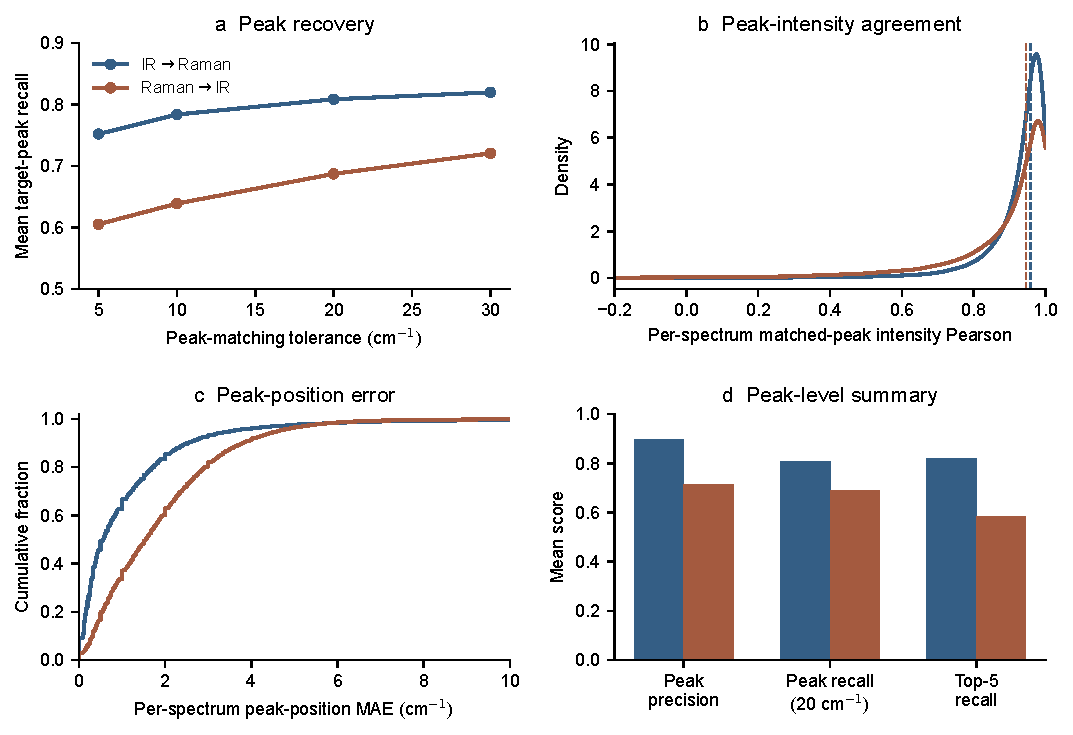
\includegraphics[width=0.88\textwidth]{figs/qm9s_bidirectional_peak_resolved.pdf}
\caption{\textbf{Bidirectional peak-resolved fidelity on the QM9S test partition.}
\textbf{a)} Mean reference-peak recall as a function of the allowed wavenumber mismatch.
\textbf{b)} Distributions of the per-spectrum Pearson correlation between normalized intensities of one-to-one matched peaks; dashed lines mark the medians.
\textbf{c)} Empirical cumulative distributions of the per-spectrum peak-position mean absolute error.
\textbf{d)} Mean peak precision, reference-peak recall at $20\,\mathrm{cm}^{-1}$ tolerance, and top-$5$ strong-peak recall. Blue denotes IR$\rightarrow$Raman and brown denotes Raman$\rightarrow$IR. All metrics are computed from $19{,}474$ held-out spectra per direction using the fixed seed-$2$ QM9S partition. The analysis uses peaks detected in broadened, per-spectrum-normalized spectra and should not be interpreted as a direct normal-mode activity evaluation.}
\label{fig:qm9s_peak_resolved}
\end{figure*}

\paragraph{Peak/non-peak partition and error profile.} For the peak- versus non-peak error comparison (Fig.~\ref{fig:case_study}c), we define \emph{peak regions} as the union of $\pm75\,\mathrm{cm}^{-1}$ windows centred on each detected \emph{target} peak, and the complementary indices as the non-peak (background) region. The reported peak/non-peak ratio is the mean normalized absolute error inside peak windows divided by the mean normalized absolute error outside them, averaged over the test set. The wavenumber-resolved error profile is the test-set mean of $|y-\hat y|$ evaluated at each wavenumber index, plotted against the mean target spectrum so that the alignment between residual mass and the target peak envelope is directly visible.

\paragraph{Peak-F1 along the trajectory.} To quantify convergence in Fig.~\ref{fig:case_study}b we track a Peak-F1 score along the flow time. At each intermediate state $x_\tau$ we detect peaks with the same relative-prominence protocol and match them against the target peaks; a predicted peak counts as a true positive when it falls within the position tolerance implied by the $\pm75\,\mathrm{cm}^{-1}$ window, and precision and recall are combined into their harmonic mean. As $\tau\rightarrow1$ the Peak-F1 rises towards one while the normalized MAE decreases, giving a trajectory-level view of how peak structure is progressively recovered.

\section{Scaffold-class definitions}\label{app:scaffold}
The scaffold breakdown in Fig.~\ref{fig:quantitative_result}d groups each test molecule by the ring system of its Bemis--Murcko scaffold~\citep{bemis1996properties}, computed with RDKit. For a given molecule, we first extract the Murcko scaffold; molecules whose scaffold contains no ring are labelled \emph{acyclic}. Ring-bearing molecules are then assigned to one of four classes according to the aromaticity and heteroatom content of their rings, evaluated over the ring systems returned by RDKit's ring perception:
\begin{itemize}
\item \textbf{Aromatic heterocycle}: at least one fully aromatic ring \emph{and} at least one ring containing a non-carbon heavy atom (e.g.\ pyridine, furan, imidazole rings).
\item \textbf{Aromatic carbocycle}: at least one fully aromatic ring, with all rings composed solely of carbon (e.g.\ benzene, naphthalene, PAHs).
\item \textbf{Aliphatic heterocycle}: no aromatic ring, but at least one ring containing a heteroatom (e.g.\ oxirane, piperidine, tetrahydrofuran rings).
\item \textbf{Aliphatic carbocycle}: no aromatic ring and all rings carbon-only (e.g.\ cyclohexane, cyclopropane rings).
\end{itemize}
A ring is deemed aromatic when all of its atoms are aromatic, and heterocyclic when any ring atom is not carbon; the aromatic test takes precedence, so a molecule containing both aromatic and heteroaromatic rings is placed in the aromatic-heterocycle class. This taxonomy is deterministic and mutually exclusive, and it captures coarse chemical distinctions, including aromaticity and heteroatom content, that are relevant to vibrational spectral structure.

To limit small-group variability, Fig.~\ref{fig:quantitative_result}d retains only classes with at least $30$ test molecules in the relevant dataset and direction, and each bar is annotated with its class size in parentheses. The same per-sample $\text{R}^2$ values used for the main results are averaged within each class; in addition to the ring-type classes above, our analysis pipeline records the exact Murcko scaffold SMILES, its generic (element-agnostic) form, the ring count, and the heavy-atom count for each molecule.
\section{Downstream probing details}\label{app:downstream}
This appendix specifies the linear-probing protocol for Fig.~\ref{fig:quantitative_result_3} and the embedding analysis in the main text.

\paragraph{Feature sets.} For each dataset and direction we compare five feature representations of every test molecule: (i) the raw source spectrum (\emph{IR raw} or \emph{Raman raw}, depending on direction), (ii) the raw target spectrum, (iii) the \mname\ \emph{Flow embedding}, (iv) a $2048$-bit Morgan fingerprint (ECFP, radius $2$), and (v) the concatenation \emph{Flow$+$fingerprint}. The Morgan fingerprint provides a strong structure-derived reference for comparison with the spectrum-derived Flow embedding, whereas the raw-source comparison tests whether the encoder makes descriptor information more accessible to a linear predictor. Raw target spectra provide an additional reference and are not required to extract the Flow embedding.

\paragraph{Flow embedding extraction.} The Flow embedding is read out from the trained velocity network without any additional training. Starting from the source spectrum we integrate the ODE to an intermediate flow time $\tau=0.5$ and mean-pool the final-block token states of the SpectraDiT backbone into a single fixed-length vector; this defines the chosen feature readout and is not evidence that the midpoint is optimal. The rollout to $\tau{=}0.5$ uses the same deterministic solver as evaluation. Because the readout is deterministic and conditioned only on the source spectrum and target-modality label, the embedding is reproducible for a given molecule.

\paragraph{Prediction targets.} The ten regression targets are RDKit-computed molecular descriptors spanning polarity, hydrogen bonding, flexibility, saturation, aromaticity, and molecular size: Crippen LogP, topological polar surface area, hydrogen-bond donor and acceptor counts, rotatable-bond count, ring count, fraction of sp$^3$ carbons, number of aromatic rings, molar refractivity, and Labute accessible surface area. Because these descriptors are deterministic functions of molecular structure, Morgan fingerprints provide a structure-derived reference for evaluating how much molecular information is linearly accessible from the spectral representation.

\paragraph{Probing model and protocol.} Each feature set is evaluated with an identical, deliberately simple probe: standardization fitted on the training partition (zero mean, unit variance), followed by ridge regression (regularization strength $\alpha=10$), to compare linear predictability under a common estimator. Feature dimensions differ, so identical probe hyperparameters do not imply identical effective capacity. Molecules with an undefined target value are dropped per property. We report $\text{R}^2$ as the mean $\pm$ standard deviation over five random train/test splits ($80/20$), with all feature sets sharing the same splits within each seed for a paired comparison. The UMAP projections in Fig.~\ref{fig:quantitative_result_3}a are for visualization only and are not used to compute any reported metric.

\section{Baseline configurations}\label{app:baselines}
The VAE and Transformer baselines are described formally in the Methods (\emph{Baseline models}); SpectraDiT-Direct is treated separately as an architecture-matched ablation. Here we give their concrete architecture and optimization settings (Supplementary Table~\ref{tab:baselines}). Both baselines consume the same spectral-map inputs and use the same train/validation/test splits as \mname. Both are trained as deterministic or variational reconstruction models without flow matching.

\paragraph{VAE.} The conditional cross-modal VAE uses a shared convolutional encoder (two stride-2 $4\times4$ convolutions with batch normalization and ReLU, widths $128$ and $256$), which is flattened and projected to a $128$-dimensional Gaussian latent via linear heads for $\mu$ and $\log\sigma^2$. A per-modality convolutional decoder (a linear layer followed by transposed convolutions back to the spectral-map resolution) reconstructs the target conditioned on the target-modality label. Training minimizes reconstruction plus $\beta\,D_{\mathrm{KL}}$, with $\beta$ raised from a small value to $\beta_{\max}=10^{-3}$ by a sigmoid KL-annealing schedule to avoid posterior collapse.

\paragraph{Transformer.} The deterministic Transformer divides the source spectral map into non-overlapping patches with a stride-$4$ convolution, embeds them as a token sequence, adds a target-modality embedding, and processes the tokens with six pre-normalized self-attention/MLP blocks (hidden width $256$, four heads, MLP ratio $4$). A normalized linear output head predicts all target patches in parallel, followed by reassembly and sigmoid projection. Optimization uses AdamW with initial learning rate $4\times10^{-4}$, weight decay $10^{-4}$, batch size $32$, and no dropout.

\begin{table}[htbp]
\centering
\caption{\textbf{Baseline configurations.} Both baselines use the same data splits and evaluation protocol as \mname; the Transformer provides a globally attentive deterministic reconstruction baseline, whereas the VAE provides a stochastic latent-variable baseline.}
\label{tab:baselines}
\begin{tabular}{@{}lll@{}}
\toprule
Model & Setting & Value \\
\midrule
\multirow{7}{*}{VAE}
 & Encoder & 2$\times$ stride-2 Conv2d ($4\times4$)$+$BN$+$ReLU \\
 & Encoder widths & $128,\ 256$ \\
 & Latent dimension $d_z$ & $128$ \\
 & Decoder & per-modality ConvTranspose2d stack \\
 & KL weight $\beta_{\max}$ & $1\times10^{-3}$ (sigmoid annealing) \\
 & Optimizer / LR & Adam / $4\times10^{-4}$ \\
 & Weight decay / batch size & $0$ / $32$ \\
\midrule
\multirow{7}{*}{Transformer}
 & Patch size $P$ & $4$ \\
 & Blocks & $6$ Transformer blocks \\
 & Hidden width $d$ & $256$ \\
 & Attention & $4$-head self-attention \\
 & Output & parallel linear patch head $+$ sigmoid \\
 & Dropout / batch size & $0.0$ / $32$ \\
 & Optimizer / LR / weight decay & AdamW / $4\times10^{-4}$ / $10^{-4}$ \\
\bottomrule
\end{tabular}
\end{table}

\end{appendices}
\clearpage

\bibliography{sn-bibliography}% common bib file
%% if required, the content of .bbl file can be included here once bbl is generated
%%\input sn-article.bbl

\end{document}
